\documentclass{tpm2026} % for initial submission
% \documentclass[accepted]{tpm2026} % after acceptance

\usepackage[american]{babel}
\usepackage{natbib} 
    \bibliographystyle{plainnat}
    \renewcommand{\bibsection}{\subsubsection*{References}}
\usepackage{mathtools} 
\usepackage{booktabs}
\usepackage{graphicx}
\usepackage{amssymb,amsmath,amsfonts,amsthm}
\usepackage{mathrsfs}
\usepackage{algorithm, algpseudocode}

\newtheorem{theorem}{Theorem}
\newtheorem{definition}{Definition}

\title{Linear Independent Component Analysis via Optimal Transport Metric as Contrast}

% The standard author block has changed for TPM 2026 to provide
% more space for long author lists and allow for complex affiliations
\author[1,2]{\href{mailto:ashutosh.jha@student.uni-tuebingen.de?Subject=TPM 2026 Paper Inquiry}{Ashutosh~Jha}}
\author[1]{Simon~Buchholz}
\author[1,3]{Michel~Besserve}
\author[2]{Joachim~Grammig}

\affil[1]{%
    Empirical Inference Group\\
    Max Planck Institute for Intelligent Systems, T\"ubingen
}
\affil[2]{%
    Chair of Statistics, Econometrics and Empirical Economics\\
    University of T\"ubingen
}
\affil[3]{%
    Institute of Artificial Intelligence\\
    TU Braunschweig
}

\begin{document}
\maketitle

\begin{abstract}
Independent Component Analysis (ICA) is a foundational probabilistic tool for recovering latent, statistically independent sources from observed mixtures. Because maximizing marginal non-Gaussianity mathematically equates to extracting independent components, traditional ICA algorithms achieve tractability by relying on local proxy contrast functions (e.g., negentropy approximations) to evaluate these non-Gaussianities. However, these proxies systematically fail to converge on complex, heterogeneous topologies. We propose OT-ICA, an exploratory framework that evaluates the full probability density by minimizing the 1D squared Wasserstein distance ($W_2^2$) to a Gaussian target. By exploiting optimal transport theory, OT-ICA retains algorithmic efficiency while demonstrating strict robustness on hybrid mixtures where traditional fixed-point solvers fail. Finally, we demonstrate the utility of this framework in two interdisciplinary applications: isolating ocular artifacts in clinical EEG recordings, and identifying structural market shocks to resolve the arbitrary recursive ordering (Cholesky) problem in standard Vector Error Correction Models (VECMs).
\end{abstract}

\section{Introduction and the Tractability Gap}
Blind source separation, specifically formulated as Independent Component Analysis (ICA) \citep{jutten1985, comon1994}, is a fundamental problem in unsupervised probabilistic modeling. The objective is to recover a set of hidden, mutually independent source signals $\mathbf{S}$ from an observed linear mixture $\mathbf{X}$. The theoretical foundation of this recovery relies on strict identifiability conditions.

\begin{theorem}[The Linear ICA Model and Identifiability \citep{comon1994}]
Let the observed data be denoted by a random vector $\mathbf{X} \in \mathbb{R}^d$, and the latent sources by $\mathbf{S} \in \mathbb{R}^d$. The linear ICA model assumes:
\begin{enumerate}
    \item \textbf{Linear Mixing:} $\mathbf{X} = \mathbf{A} \mathbf{S}$, where $\mathbf{A} \in \mathbb{R}^{d \times d}$ is an unknown, invertible mixing matrix.
    \item \textbf{Independence:} The components $s_1, \dots, s_d$ of $\mathbf{S}$ are mutually statistically independent.
    \item \textbf{Non-Gaussianity:} At most one of the source components $s_i$ follows a Gaussian distribution.
\end{enumerate}
Under these conditions, the mixing matrix $\mathbf{A}$ can be uniquely identified from the observations $\mathbf{X}$, up to a permutation and scaling of its columns.
\end{theorem}

Because of the Central Limit Theorem, mixtures of independent non-Gaussian variables are mathematically more Gaussian than the constituent sources. Standard ICA isolates these sources by navigating the space of orthogonal rotation matrices to maximize the non-Gaussianity of the projected data \citep{hyvarinen2001}. This heuristic search is mathematically rigorous, as formalized by information geometry.

\begin{theorem}[Equivalence of Independence and Non-Gaussianity \citep{cardoso2022}]
Let $Y$ be a zero-mean random vector with an identity covariance matrix (whitened). 
The mutual information $\mathscr{I}(Y)$ is directly determined by the joint non-Gaussianity $G(Y)$ and the sum 
of marginal non-Gaussianities $\sum_i G(Y_i)$ via the strict relationship:
\begin{equation}
    \mathscr{I}(Y) = G(Y) - \sum_{i} G(Y_i)
\end{equation}
Because joint non-Gaussianity $G(Y)$ is invariant under orthogonal rotation, minimizing mutual information (extracting independent components) is mathematically equivalent to maximizing the sum of marginal non-Gaussianities.
\end{theorem}
\textit{(A comprehensive proof of this theorem using Kullback-Leibler Pythagorean identities on the Product and Gaussian manifolds is provided in Appendix \ref{app:info_geometry}.)}

However, evaluating the full density of a continuous distribution to measure non-Gaussianity is computationally expensive. To remain tractable, classical algorithms such as FastICA \citep{hyvarinen2001, amari1996new}, InfoMax \citep{bell1995information}, and JADE \citep{cardoso1993blind} rely on surrogate information-theoretic contrast functions (e.g., \textit{logcosh} approximations, log-likelihood surrogates, and fourth-order cumulants). Consequently, they fail to capture the global geometry of underlying distributions, leading to optimization failures in heterogeneous mixtures (detailed in Appendix \ref{app:proxy_limits}).

While the 1D $W_2$ distance has been studied as a Gaussianity measure in statistical testing \citep{delbarrio1999} and Sliced Wasserstein methods leverage 1D marginal projections for general distribution comparison \citep{peyre2019computational}, no prior work formalizes $W_2^2$-to-Gaussian as a blind source separation contrast backed by identifiability theory.
To bridge this gap, we explore OT-ICA. In optimal transport theory, the Monge problem \citep{monge1781} and its Kantorovich relaxation \citep{kantorovich1942} define the general Wasserstein distance $W_p$ \citep{villani2003} between a source measure $\mu$ and a target $\nu$ over the space of optimal probabilistic couplings $\Pi(\mu, \nu)$ as:
\begin{equation}
    W_p(\mu, \nu) = \left( \inf_{\pi \in \Pi(\mu, \nu)} \int \|x - y\|^p \, d\pi(x, y) \right)^{1/p}
\end{equation}
While calculating this coupling is intractable in high dimensions, in the 1D setting data can be unambiguously sorted. By Brenier's Theorem \citep{brenier1991} and Caffarelli's regularity theory \citep{caffarelli1992}, the 1D transport map is monotonic. Consequently, the squared Wasserstein distance ($p=2$) analytically collapses to the integrated squared difference between the inverse cumulative distribution functions (quantile functions):
\begin{equation}
    W_2^2(\mu, \nu) = \int_0^1 |F_\mu^{-1}(t) - F_\nu^{-1}(t)|^2 \, dt
\end{equation}
By relying strictly on 1D projections, OT-ICA provides a highly tractable, proxy-free metric capable of robust structural identification. 

\section{The Exploratory OT-ICA Framework}

Once observed data $\mathbf{X}$ is centered and whitened to yield unit-variance and uncorrelated components $\widetilde{\mathbf{X}}$, the search for independent components is strictly constrained to the Orthogonal Group $\mathcal{S}$ \citep{cardoso2022}. The OT-ICA objective is to find the orthogonal projection $\mathbf{b}$ that maximizes the distance to the standard normal distribution $\Gamma \equiv \mathcal{N}(0,1)$:
\begin{equation}
    \hat{\mathbf{b}} = \arg\max_{\mathbf{b} \in \mathcal{S}} W_2^2\big(\mathbb{P}_{\mathbf{b}^\top \widetilde{\mathbf{X}}}, \Gamma\big).
\end{equation}

This optimization is mathematically justified by bounding the non-Gaussianity of the mixture. 

\begin{theorem}[$W_2$ Upper Bound]
Let $\mathbf{Z} = (Z_1, \dots, Z_d)^\top$ be a vector of mutually independent latent sources, and let $\mathbf{b}$ be a weight vector on the unit sphere ($\sum_{i=1}^d b_i^2 = 1$). The squared Wasserstein distance between the linear mixture $\mathbf{b} \cdot \mathbf{Z}$ and the standard normal distribution $\Gamma$ is bounded by the weighted sum of the source distances to $\Gamma$:
\begin{equation}
    W_2^2(\mathbf{b} \cdot \mathbf{Z}, \Gamma) \le \sum_{i=1}^d b_i^2 W_2^2(Z_i, \Gamma).
\end{equation}
\end{theorem}

\begin{theorem}[Strict $W_2$ Inequality for Non-Gaussian Sources]
Assuming at most one source $Z_i$ is Gaussian, and the source distributions possess smooth and strictly positive densities, the upper bound derived in Theorem 3 is a strict inequality for any valid mixture where multiple weights $b_i$ are non-zero:
\begin{equation}
    W_2^2(\mathbf{b} \cdot \mathbf{Z}, \Gamma) < \sum_{i=1}^d b_i^2 W_2^2(Z_i, \Gamma).
\end{equation}
\end{theorem}

Because the mixture is strictly less non-Gaussian than its parts, finding the global maximum forces the weight vector to collapse to a canonical axis, successfully isolating the independent component. \textit{(The full mathematical proofs of these inequalities, demonstrating comonotonicity contradictions under Caffarelli's regularity theory, are provided in Appendix \ref{app:proofs}).}

\subsection{Methodological Enhancements}
While 1D optimal transport allows for a tractable $\mathcal{O}(N \log N)$ empirical sorting operation, optimizing this metric efficiently and robustly requires specific algorithmic enhancements: 
1) \textbf{Analytical Gaussian Targets} to eliminate discrete sampling noise \citep{fournier2015rate}; 
2) \textbf{Riemannian Gradient} projection and \textbf{Symmetric Decorrelation Retraction} to navigate the non-Euclidean Stiefel manifold without violating independence constraints \citep{absil2008optimization}; and 
3) \textbf{Gaussian Dithering} to smooth zero-gradient plateaus in discrete domains \citep{schuchman1964dither}. 

A discussion on why $W_2^2$ provides smoother optimization gradients than $W_1$, alongside the complete theoretical formulations, definitions, complexity analysis, and the full stochastic Riemannian optimization pseudocode for the algorithm are detailed in Appendix \ref{app:methodology}.

\section{OT-ICA Methodology Validation}
To empirically evaluate the success of source separation, we quantify the structural distance between the estimated unmixing matrix $\mathbf{B}_{\text{est}}$ and the true mixing matrix $\mathbf{A}$. Because ICA is fundamentally subject to scaling and permutation ambiguities (as defined in Theorem 1), perfect unmixing mathematically results in a \textit{generalized permutation matrix} $\mathbf{P} = \mathbf{B}_{\text{est}}\mathbf{A} \in \mathcal{P}$, where $\mathcal{P}$ is the set of matrices with exactly one non-zero entry in each row and column. 

We quantify this convergence using the Amari Performance Index ($E$) \citep{amari1996new}, a standardized metric that measures the deviation of the gain matrix $\mathbf{P}$ from the nearest permutation matrix. An index of $E < 0.1$ indicates near-perfect separation, while $E \ge 0.5$ indicates a failure to unmix the signals (full formal definitions and experimental regimes are provided in Appendix \ref{app:experimental_setup}).

\begin{figure}[htbp]
    \centering
    
\includegraphics[width=1.0\columnwidth]{otica_baseline_recovery.pdf}
    \caption{Baseline validation of OT-ICA convergence on standard continuous mixtures. The squared Wasserstein distance ($W_2^2$) acts as a smooth contrast, driving the Amari error toward zero.}
    \label{fig:ot_ica_validation}
\end{figure}

Baseline testing (Figure \ref{fig:ot_ica_validation}) confirms that the $W_2^2$ gradient reliably drives the Amari error toward zero on standard continuous mixtures (such as symmetric Laplacian signals), empirically validating the structural convergence of the Riemannian manifold traversal and the analytical targets.

\section{Empirical Robustness on Hybrid Mixtures}
Following baseline validation, we evaluate the general robustness of OT-ICA against FastICA.

\begin{figure}[htbp]
    \centering
    
\includegraphics[width=0.95\columnwidth]{general_hybrid_test.pdf}
    \caption{Amari error for Generalized Hybrid Mixtures. OT-ICA demonstrates reliable stability across tested dimensions compared to FastICA.}
    \label{fig:hybrid_mixture_results}
\end{figure}

For our primary evaluation, we simulated heterogeneous environments mixing a standard Gaussian with $(d-1)$ randomly drawn independent sources covering super-Gaussian, sub-Gaussian, continuous, and discrete distributions (e.g., Laplace, Bernoulli, Uniform, Poisson, Exponential). 

Figure \ref{fig:hybrid_mixture_results} confirms that FastICA exhibits severe instability in multi-modal, hybrid environments, frequently failing to converge (Amari Error $> 0.5$). By utilizing a true geometric distance metric that evaluates the full probability density rather than a local approximation, OT-ICA provides stable separation across complex mixed topologies. (Extended evaluations regarding computational scaling and dimensionality limits are discussed in Appendix \ref{app:scaling}).

\section{Interdisciplinary Applications}

\subsection{Structural Identification in Price Discovery}
In fragmented financial markets, identical assets traded across venues are bound together by an unobserved random walk. Modeling these price dynamics heavily relies on Vector Error Correction Models (VECMs) \citep{engle1987, johansen1991}. To determine the Information Share (IS) \citep{hasbrouck1995, baillie2002} of each market, the reduced-form residuals $u_t$ must be decomposed into mutually independent structural shocks $\epsilon_t$ via an impact matrix $\mathbf{B}$ such that $u_t = \mathbf{B} \epsilon_t$.

Since $\boldsymbol{\Omega} = \mathbf{B}\mathbf{B}^\top$ only partially identifies $\mathbf{B}$, standard Cholesky decomposition imposes an arbitrary recursive market ordering, yielding drastically different IS estimates depending on the market vector's arrangement.

To achieve unique, order-invariant identification, $\mathbf{B}$ can be factored as $\mathbf{B} = \mathbf{S}\mathbf{C}$, where $\mathbf{S}$ is an arbitrary whitening matrix and $\mathbf{C}$ is a strict orthogonal rotation. This transforms the price discovery problem into a search for $\mathbf{C}$ \citep{zema2025}. Applying OT-ICA leverages the heavy-tailed non-Gaussianity of financial innovations to explicitly lock $\mathbf{C}$, recovering the true structural shocks without imposing Cholesky's recursive assumptions.

\begin{table}[htbp]
    \centering
    \resizebox{\columnwidth}{!}{
    \begin{tabular}{@{}lccc@{}}
        \toprule
        \textbf{Market / Source} & \textbf{True IS} & \textbf{Estimated IS (Mean)} & \textbf{Std. Dev.} \\
        \midrule
        Market 1 & 0.1200 & 0.1212 & 0.0161 \\
        Market 2 & 0.2400 & 0.2399 & 0.0245 \\
        Market 3 & 0.6400 & 0.6389 & 0.0260 \\
        \bottomrule
    \end{tabular}
    }
    \caption{Simulation Results for Information Share Recovery across 500 Monte Carlo runs. The estimated IS tightly matches the true IS without imposing arbitrary Cholesky recursive structures.}
    \label{tab:simulated_is_results}
\end{table}

As shown in Table \ref{tab:simulated_is_results}, OT-ICA successfully identifies the independent driving shocks, achieving mean IS estimates tightly converging to the true generative parameters (12.1\%, 23.9\%, 63.8\%).

\subsection{EEG Artifact Removal}
In electroencephalography, the human skull acts as a linear volume conductor \citep{hyvarinen2001} where ocular artifacts (blinks) mix linearly with brain waves before reaching the scalp electrodes. Because blinks are highly sparse and super-Gaussian, OT-ICA naturally identifies and isolates them.

\begin{figure}[htbp]
    \centering
    
\includegraphics[width=0.95\columnwidth]{eeg_artifact_removal.pdf}
    \caption{OT-ICA isolating ocular artifacts (Comp 1) from five raw frontal EEG channels, enabling downstream neuro-scientific analysis.}
    \label{fig:eeg_artifact}
\end{figure}

As demonstrated in Figure \ref{fig:eeg_artifact}, OT-ICA successfully filters the synchronized high-amplitude spikes into a single independent component, preserving the underlying brain wave structures.

\section{Conclusion}
By formulating ICA as a tractable 1D optimal transport problem, OT-ICA overcomes the geometric limitations of classical proxy contrast solvers. We demonstrated its robustness across heterogeneous mixtures and its specific utility in resolving structural ordering ambiguities in VECM models and isolating clinical artifacts. Future work will integrate OT-ICA directly into Causal Discovery frameworks, specifically extending Linear Non-Gaussian Acyclic Models (LiNGAM) \citep{shimizu2006linear} and Causal Component Analysis (CauCA) \citep{liang2023causal} to improve causal representation learning in highly complex distributions.

\bibliography{tpm2026-template}

\newpage
\onecolumn
\appendix

\begin{center}
    \Large\textbf{Supplementary Material for:}\\
    \large\textbf{Linear Independent Component Analysis via Optimal Transport Metric as Contrast}
\end{center}

\section{Information Geometry of ICA}
\label{app:info_geometry}
Information geometry provides a framework for quantifying the relationship between independence and non-Gaussianity by analyzing probability distributions as points on geometric manifolds. Following the perspective introduced by \citet{cardoso2022}, ICA can be understood as orthogonally projecting the empirical distribution $P_Y$ onto two distinct subspaces: the Product manifold $\mathcal{P}$ (containing distributions where marginals are strictly independent) and the Gaussian manifold $\mathcal{G}$ (encompassing all multivariate Gaussians). 

\begin{figure}[htbp]
    \centering
    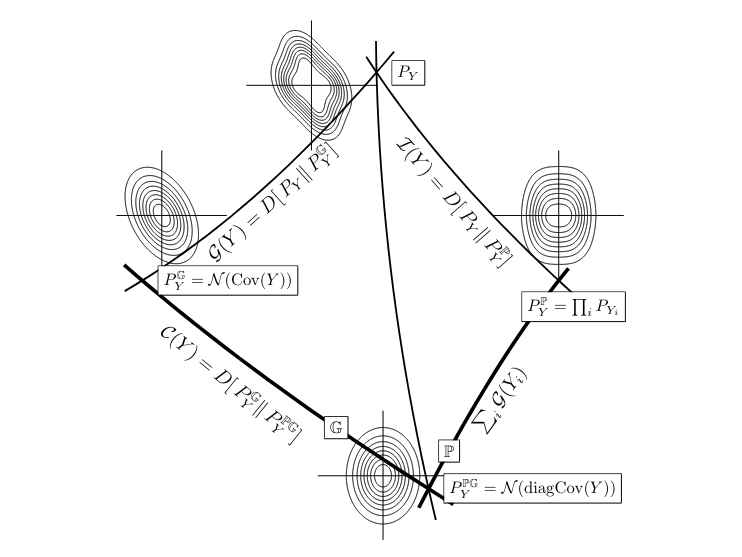
\includegraphics[width=0.75\textwidth]{pythagorean_ig_ica.png}
    \caption{The Pythagorean geometry of Independent Component Analysis. Figure from \citet{cardoso2022}.}
    \label{fig:cardoso_geometry}
\end{figure}

The Mutual Information $\mathscr{I}(Y)$ measures the distance from $P_Y$ to its closest independent product distribution $P_Y^P$. A Pythagorean identity exists on the Product manifold for any candidate product distribution $Q = \prod_{i} q_i$:
\begin{align}\label{eq:pythagoras_product}
    D_{\mathrm{KL}}\left(P_Y \Vert Q\right) &= \int P_Y(y) \log \left( \frac{P_Y(y)}{P_Y^P(y)} \frac{P_Y^P(y)}{Q(y)} \right) dy \nonumber \\
    &= \mathscr{I}(Y) + \sum_{i} D_{\mathrm{KL}}\left(P_{Y_i} \Vert q_i\right).
\end{align}

A similar Pythagorean identity holds for the Gaussian manifold $\mathcal{G}$. Let $\Phi_Y = \mathcal{N}(0, \operatorname{Cov} Y)$ be the best Gaussian fit (sharing the exact mean and covariance of $P_Y$), and let $\Phi = \mathcal{N}(0, \Sigma)$ be an arbitrary Gaussian target. The divergence decomposes as:
\begin{align}
    D_{\mathrm{KL}}\big(P_Y \Vert \Phi\big) &= \int P_Y(y) \log \left( \frac{P_Y(y)}{\Phi_Y(y)} \frac{\Phi_Y(y)}{\Phi(y)} \right) dy \nonumber \\
    &= \int P_Y(y) \log \frac{P_Y(y)}{\Phi_Y(y)} dy + \int P_Y(y) \log \frac{\Phi_Y(y)}{\Phi(y)} dy \nonumber \\
    &= D_{\mathrm{KL}}\big(P_Y \Vert \Phi_Y\big) + \mathbb{E}_{P_Y}\left[ \log \Phi_Y(y) - \log \Phi(y) \right].
\end{align}

Because the log-density of a zero-mean Gaussian is a quadratic form, its expectation strictly depends only on the second moments (the covariance matrix) of the variable. Since the true distribution $P_Y$ and its Gaussian fit $\Phi_Y$ share the exact same covariance matrix by definition, evaluating the expectation of this quadratic form under $P_Y$ is mathematically identical to evaluating it under $\Phi_Y$:
\begin{equation}
    \mathbb{E}_{P_Y}\left[ \log \frac{\Phi_Y(y)}{\Phi(y)} \right] = \mathbb{E}_{\Phi_Y}\left[ \log \frac{\Phi_Y(y)}{\Phi(y)} \right] = D_{\mathrm{KL}}\big(\Phi_Y \Vert \Phi\big).
\end{equation}

Substituting this equivalence back establishes the Pythagorean identity on the Gaussian manifold:
\begin{equation}\label{eq:pythagoras_gaussian}
    D_{\mathrm{KL}}\big(P_Y \Vert \mathcal{N}(\Sigma)\big) = D_{\mathrm{KL}}\big(P_Y \Vert \mathcal{N}(\operatorname{Cov} Y)\big) + D_{\mathrm{KL}}\big(\mathcal{N}(\operatorname{Cov} Y) \Vert \mathcal{N}(\Sigma)\big).
\end{equation}

We define the joint non-Gaussianity as $G(Y) = D_{\mathrm{KL}}(P_Y \,\Vert\, \mathcal{N}(\operatorname{Cov} Y))$, and correlation as $C(Y) = D_{\mathrm{KL}}(\mathcal{N}(\operatorname{Cov} Y) \,\Vert\, \mathcal{N}(\operatorname{diag\,Cov} Y))$. By evaluating the KL divergence from $P_Y$ to a fully factorized Gaussian target $\mathcal{N}(\operatorname{diag\,Cov} Y)$ via both the Product path and Gaussian path, we yield Cardoso's unified theorem \citep{cardoso2022}:
\begin{equation}
    \mathscr{I}(Y) + \sum_{i} G(Y_i) = G(Y) + C(Y).
\end{equation}

Crucially, once the data is whitened ($\operatorname{Cov}(Y) = \mathbf{I}$), correlation drops strictly to zero ($C(Y) = 0$). The relationship rearranges strictly as:
\begin{equation}
    \mathscr{I}(Y) = G(Y) - \sum_{i} G(Y_i).
\end{equation}
Because joint non-Gaussianity $G(Y)$ is invariant under orthogonal rotation, minimizing mutual information (achieving independence) mathematically equates exactly to maximizing the sum of marginal non-Gaussianities $\sum G(Y_i)$.

\section{Mathematical Proofs for OT-ICA Bounds}
\label{app:proofs}

\subsection{Proof of Theorem 3: $W_2$ Upper Bound}
\begin{theorem}[$W_2$ Upper Bound]
Let $\mathbf{Z} = (Z_1, \dots, Z_d)^\top$ be a vector of mutually independent latent sources, and let $\mathbf{b}$ be a weight vector on the unit sphere ($\sum_{i=1}^d b_i^2 = 1$). The squared Wasserstein distance between the linear mixture $\mathbf{b} \cdot \mathbf{Z}$ and the standard normal distribution $\Gamma$ is bounded by the weighted sum of the source distances to $\Gamma$:
\begin{equation}
    W_2^2(\mathbf{b} \cdot \mathbf{Z}, \Gamma) \le \sum_{i=1}^d b_i^2 W_2^2(Z_i, \Gamma).
\end{equation}
\end{theorem}

\textit{Proof.} We construct a specific joint probability distribution, or coupling, using a common source of randomness. Let $\mathbf{N} = (N_1, \dots, N_d)^\top$ be a vector of $d$ independent standard normal variables, $\mathbf{N} \sim \mathcal{N}(0, \mathbf{I}_d)$, assumed to be statistically independent of the sources $\mathbf{Z}$. For each independent latent source $Z_i$, there exists an optimal transport map $T_i$ that pushes forward the standard normal distribution to the source distribution, denoted as $(T_i)_{\#} \Gamma = Z_i$. 

We construct a random variable $X$ representing the mixture:
\begin{equation}
    X = \sum_{i=1}^d b_i T_i(N_i).
\end{equation}
To compare this mixture to a Gaussian distribution, we construct a target variable $Y$ using the same underlying noise vector $\mathbf{N}$:
\begin{equation}
    Y = \sum_{i=1}^d b_i N_i.
\end{equation}
Given that the weights sum to unity, the resulting variable $Y$ follows the standard normal distribution, $Y \sim \Gamma$. The pair $(X, Y)$ creates a valid coupling. Because $W_2^2$ is the infimum over all valid couplings, the optimal distance is less than or equal to the cost of our constructed coupling:
\begin{equation}
    W_2^2(\mathbf{b} \cdot \mathbf{Z}, \Gamma) \le \mathbb{E}\left[|X - Y|^2\right] = \mathbb{E}\left[ \left( \sum_{i=1}^d b_i \big(T_i(N_i) - N_i\big) \right)^2 \right].
\end{equation}
Squaring the summation produces diagonal terms ($i=j$) and cross terms ($i \neq j$):
\begin{equation}
    |X - Y|^2 = \sum_{i=1}^d b_i^2 \big(T_i(N_i) - N_i\big)^2 + \sum_{i \neq j} b_i b_j \big(T_i(N_i) - N_i\big)\big(T_j(N_j) - N_j\big).
\end{equation}
Because the underlying noise variables $N_i$ and $N_j$ are independent, and the functions evaluate to a mean of zero, when we take the expectation, all cross terms vanish. We are left with the expectation of the diagonal terms:
\begin{equation}
    \mathbb{E}\left[|X - Y|^2\right] = \sum_{i=1}^d b_i^2 \mathbb{E}\left[ \big(T_i(N_i) - N_i\big)^2 \right].
\end{equation}
Recognizing that $\mathbb{E}[ (T_i(N_i) - N_i)^2 ]$ is the definition of the squared Wasserstein distance between the individual source $Z_i$ and $\Gamma$, we arrive at the bound:
\begin{equation}
    W_2^2(\mathbf{b} \cdot \mathbf{Z}, \Gamma) \le \sum_{i=1}^d b_i^2 W_2^2(Z_i, \Gamma). \quad \blacksquare
\end{equation}

\subsection{Proof of Theorem 4: Strict Inequality}
\begin{theorem}[Strict $W_2$ Inequality for Non-Gaussian Sources]
Assuming at most one source $Z_i$ is Gaussian, and the source distributions possess smooth and strictly positive densities, the upper bound derived in Theorem 3 is a strict inequality for any valid mixture where multiple weights $b_i$ are non-zero:
\begin{equation}
    W_2^2(\mathbf{b} \cdot \mathbf{Z}, \Gamma) < \sum_{i=1}^d b_i^2 W_2^2(Z_i, \Gamma).
\end{equation}
\end{theorem}

\textit{Proof.} In a one-dimensional setting, the $W_2$ distance equals the expected squared difference of a specific coupling if and only if the random variables are comonotonic. By Brenier's Theorem \citep{brenier1991}, this requires the gradients to be parallel at every point in the probability space:
\begin{equation}
    \nabla X(\mathbf{N}) = \lambda(\mathbf{N}) \nabla Y(\mathbf{N}).
\end{equation}
Assuming the source distributions possess smooth and strictly positive densities, Caffarelli's regularity theory \citep{caffarelli1992} guarantees that the optimal transport maps $T_i$ are continuously differentiable. 

We differentiate both sides to compute their Hessian matrices. On the LHS, the cross-derivatives $\frac{\partial^2 X}{\partial N_i \partial N_j}$ are zero, yielding a diagonal matrix of $b_i T''_i(N_i)$. On the RHS, we differentiate the product $\lambda(\mathbf{N}) \mathbf{b}$, yielding a Rank-1 outer product matrix:
\begin{equation}
    \underbrace{
    \begin{bmatrix} 
    b_1 T''_1(N_1) & 0 & \cdots & 0 \\
    0 & b_2 T''_2(N_2) & \cdots & 0 \\
    \vdots & \vdots & \ddots & \vdots \\
    0 & 0 & \cdots & b_d T''_d(N_d)
    \end{bmatrix}
    }_{\text{Hessian of } X \text{ (Diagonal)}}
    =
    \underbrace{
    \begin{bmatrix}
    b_1 \frac{\partial \lambda}{\partial N_1} & \cdots & b_1 \frac{\partial \lambda}{\partial N_d} \\
    \vdots & \ddots & \vdots \\
    b_d \frac{\partial \lambda}{\partial N_1} & \cdots & b_d \frac{\partial \lambda}{\partial N_d}
    \end{bmatrix}
    }_{\text{Outer Product } \mathbf{b} (\nabla \lambda)^\top \text{ (Rank-1)}}
\end{equation}
Examining any off-diagonal entry ($i \neq j$), the LHS dictates it must be zero, establishing $b_i \frac{\partial \lambda}{\partial N_j} = 0$. Because we assume a mixture where multiple weights are non-zero ($b_i \neq 0$), it follows that the gradient of the scaling function is zero ($\nabla \lambda = \mathbf{0}$). Consequently, $\lambda(\mathbf{N})$ is a global scalar constant, $\lambda$.

Equating the diagonal elements implies $T'_i(N_i) = \lambda$. Integrating this indicates the optimal transport maps are linear functions of the form:
\begin{equation}
    T_i(x) = \lambda x + c.
\end{equation}
Applying a purely linear transformation to Gaussian noise $N_i$ produces another Gaussian distribution. The identifiability assumption of ICA dictates that the original latent sources $Z_i$ are non-Gaussian. Therefore, the linear map requirement contradicts the non-Gaussianity of the sources. Because the condition for equality cannot be met, the relationship is a strict inequality. $\blacksquare$

\subsection{Proof of Intractability of Newton Updates for Empirical OT-ICA}
\begin{theorem}[Intractability of Newton Updates]
For an empirical distribution mapped to a continuous target via sorting, computing a closed-form Hessian $\mathbf{H} = \nabla^2_{\mathbf{b}} W_2^2$ is analytically intractable without introducing external density estimation mechanisms. The Map Derivative $\nabla_{\mathbf{b}} T_{\mathbf{b}}$ strictly requires the continuous Probability Density Function (PDF) evaluated at the quantile boundaries.
\end{theorem}

\textit{Proof.} To implement a fixed-point Newton step, the Hessian matrix of the squared Wasserstein distance, $\mathbf{H} = \nabla^2_{\mathbf{b}} W_2^2$, is required. Let the 1D projection of the data be $y = \mathbf{b}^\top \mathbf{X}$, and let $T_{\mathbf{b}}$ be the optimal transport map pushing this empirical projection to the target Gaussian distribution. 

We compute the first differential (the gradient) with respect to $\mathbf{b}$. Utilizing the envelope theorem for optimal transport, the variation of the optimal map evaluates to zero within the cost function:
\begin{align}
    \mathbf{g} = \nabla_{\mathbf{b}} \left( \frac{1}{2} W_2^2 \right) &= \mathbb{E}\Big[ \mathbf{X} \big( \mathbf{b}^\top \mathbf{X} - T_{\mathbf{b}}(\mathbf{b}^\top \mathbf{X}) \big) \Big].
\end{align}

To compute the Hessian $\mathbf{H}$, we must differentiate the gradient vector $\mathbf{g}$ with respect to $\mathbf{b}$:
\begin{align}
    \mathbf{H} = \nabla_{\mathbf{b}} \mathbf{g} &= \mathbb{E}\Big[ \mathbf{X} \mathbf{X}^\top - \mathbf{X} \nabla_{\mathbf{b}} [T_{\mathbf{b}}(\mathbf{b}^\top \mathbf{X})]^\top \Big].
\end{align}

Applying the total derivative using the chain rule yields two distinct components:
\begin{equation}
    \nabla_{\mathbf{b}} [T_{\mathbf{b}}(\mathbf{b}^\top \mathbf{X})] = \underbrace{T'_{\mathbf{b}}(\mathbf{b}^\top \mathbf{X}) \mathbf{X}}_{\text{Argument Derivative}} + \underbrace{(\nabla_{\mathbf{b}} T_{\mathbf{b}})(\mathbf{b}^\top \mathbf{X})}_{\text{Map Derivative}}.
\end{equation}
By Caffarelli's regularity theory \citep{caffarelli1992}, the transport map $T_{\mathbf{b}}$ is continuously differentiable, guaranteeing the existence of the Argument Derivative. The fundamental limitation lies within the Map Derivative. 

In the 1D optimal transport setting, the transport map relies on the empirical cumulative distribution function, $F_{\mathbf{b}}$, of the projected data $y$. Expanding the Map Derivative yields:
\begin{equation}
    (\nabla_{\mathbf{b}} T_{\mathbf{b}})(y) = \nabla_{\mathbf{b}} \big[ \Phi^{-1}(F_{\mathbf{b}}(y)) \big] = \frac{1}{\phi(\Phi^{-1}(F_{\mathbf{b}}(y)))} \nabla_{\mathbf{b}} F_{\mathbf{b}}(y).
\end{equation}
The term $\nabla_{\mathbf{b}} F_{\mathbf{b}}(y)$ represents the rate of change of the cumulative probability mass as the projection plane $\mathbf{b}$ is rotated. The derivative of a cumulative distribution function's boundary strictly requires the underlying continuous probability density function (PDF) evaluated at that specific boundary. For empirical distributions consisting of discrete sampled points, this density does not natively exist, rendering the closed-form calculation of the Hessian analytically intractable. $\blacksquare$

\section{Algorithmic Enhancements and Methodology}
\label{app:methodology}

\subsection{Why $W_2^2$ Instead of $W_1$?}
While the $W_1$ distance is robust to outliers, its reliance on an absolute $L_1$ penalty introduces severe geometric challenges on finite samples. 

\begin{figure}[htbp]
    \centering
    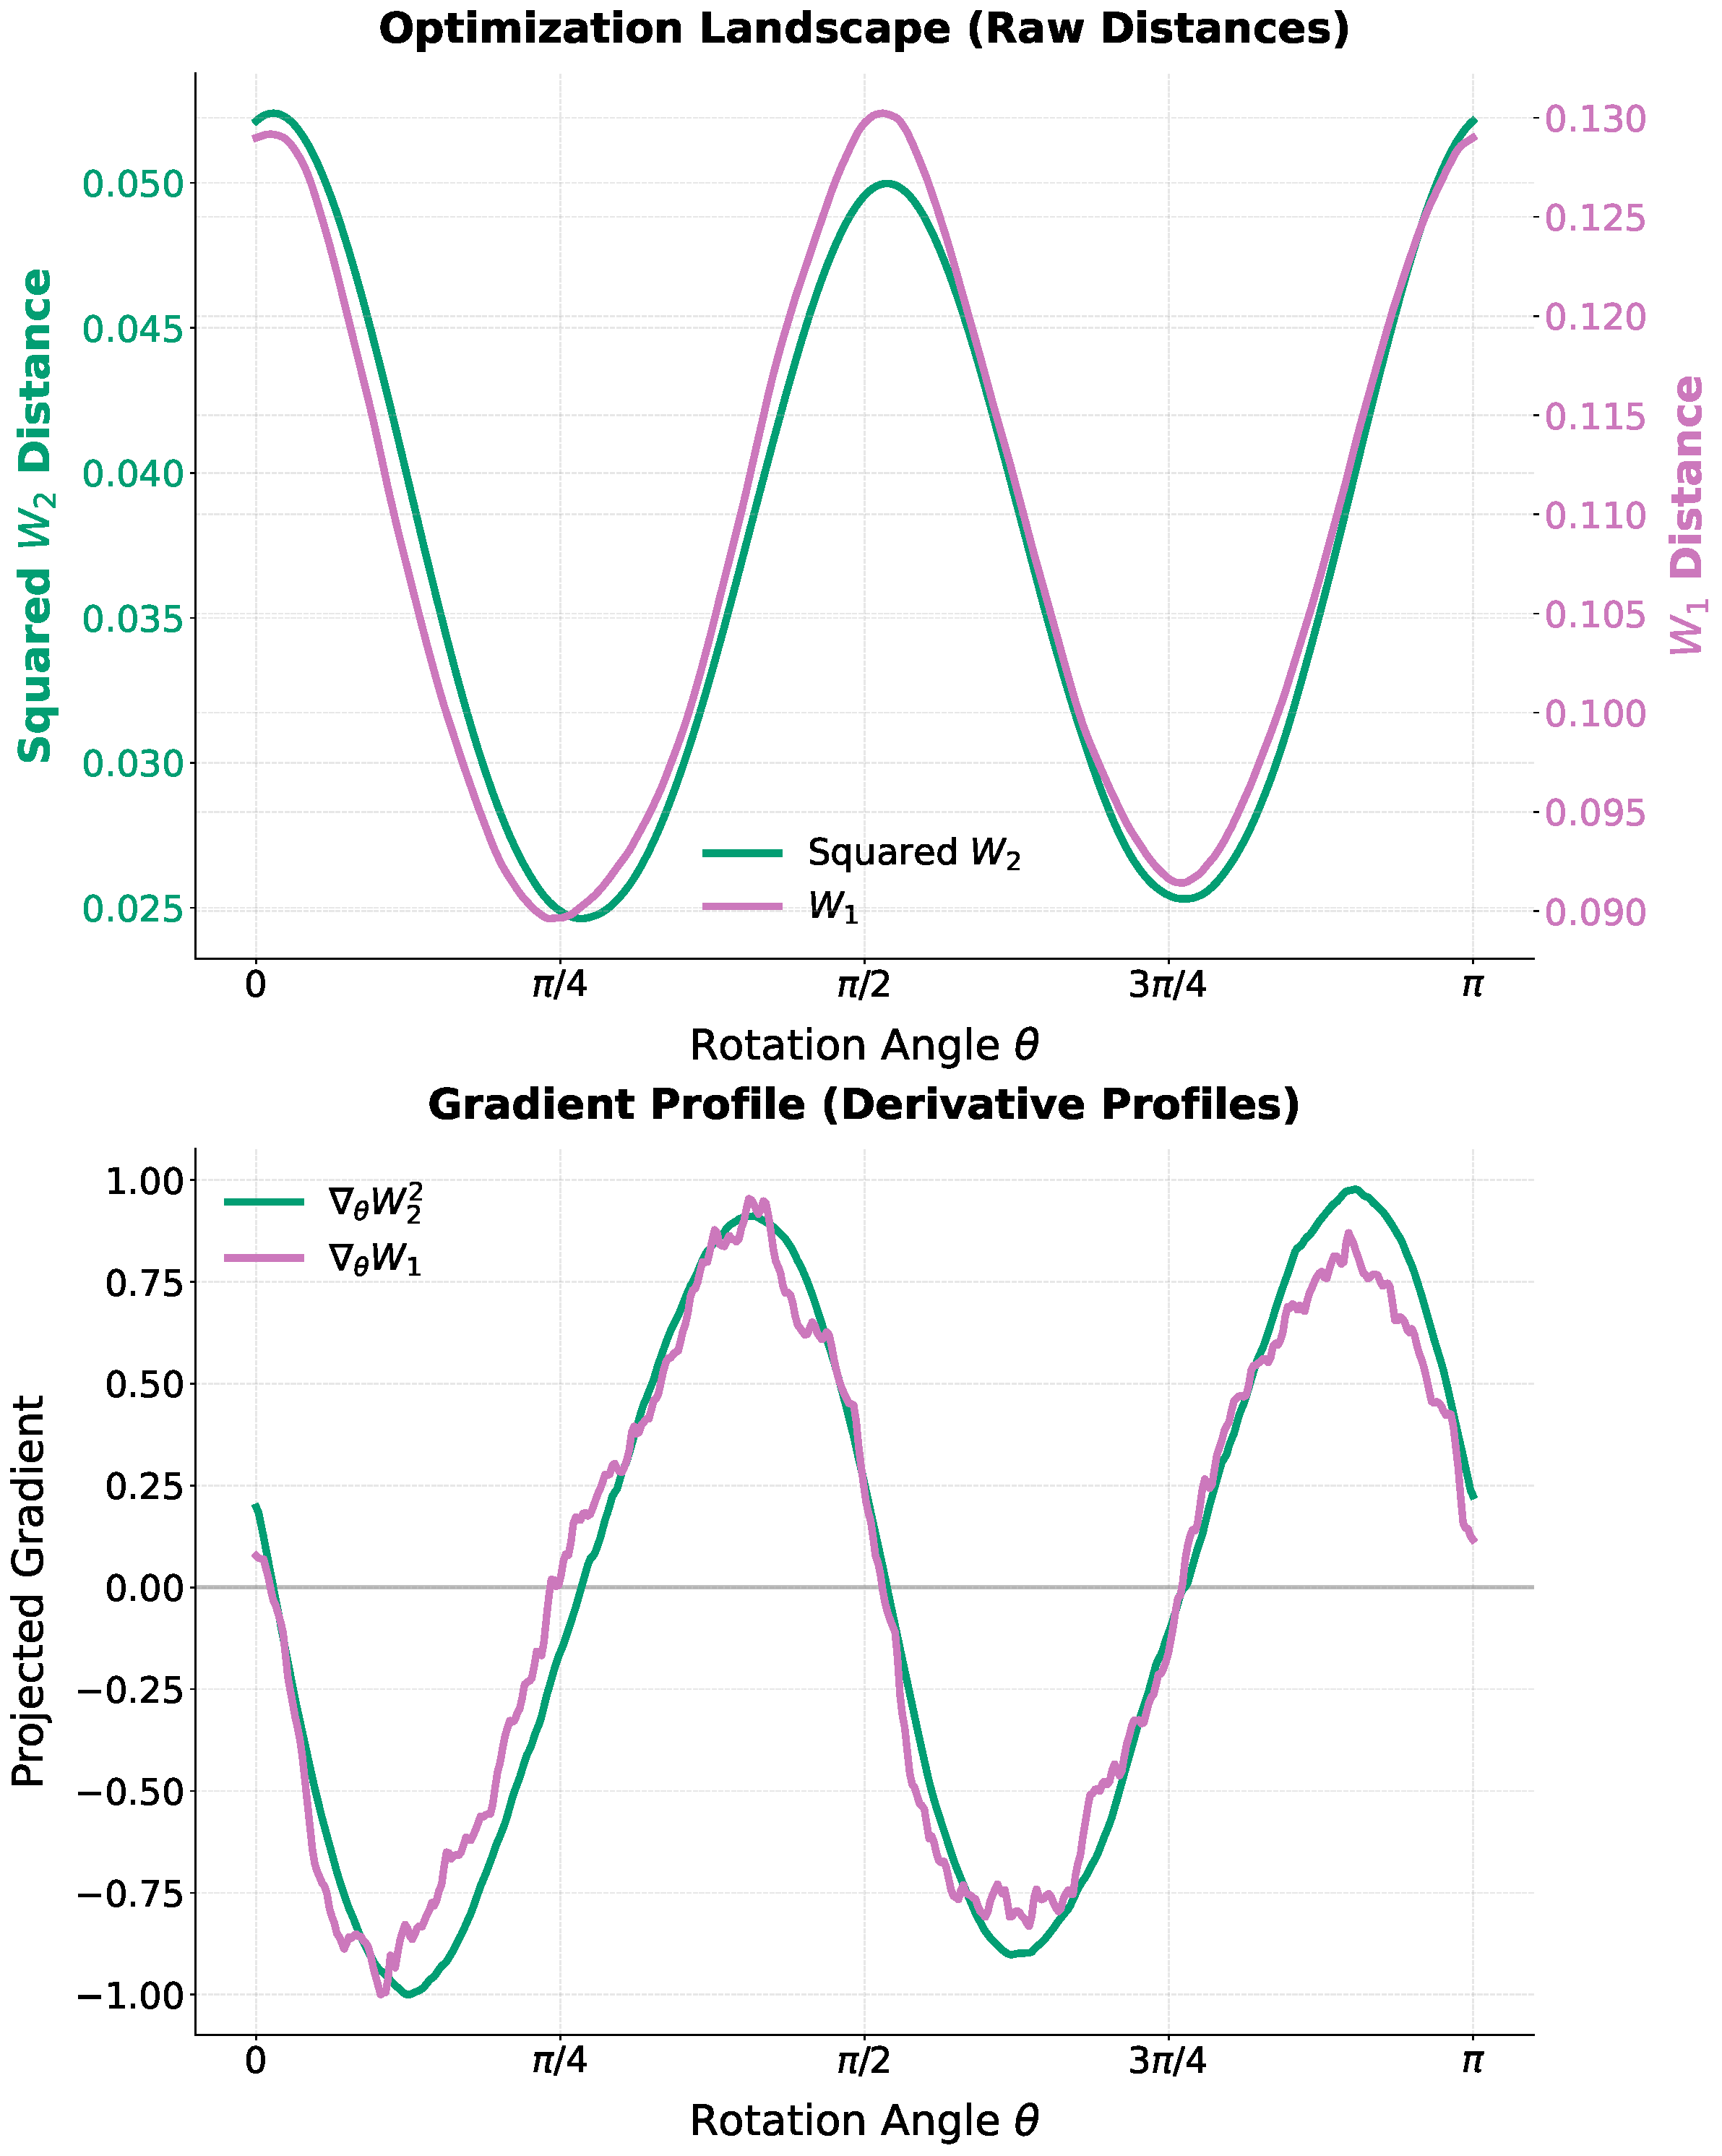
\includegraphics[width=0.9\textwidth]{w1_vs_w2_derivatives.pdf}
    \caption{Gradient Landscapes of $W_1$ and $W_2^2$ across continuous rotation angles $\theta$. The $W_2^2$ gradient smoothly decelerates toward zero, whereas the $W_1$ gradient exhibits jagged volatility on finite empirical samples.}
    \label{fig:w1_vs_w2_derivatives}
\end{figure}

As shown in Figure \ref{fig:w1_vs_w2_derivatives}, the $W_1$ cost lacks the convexity needed to smooth out empirical noise. Its derivative fluctuates frequently, causing first-order gradient ascent solvers to stall in local non-smooth traps. The squared penalty in the $W_2^2$ metric acts as a structural smoother, penalizing local distortions and providing a continuous, decelerating gradient profile that allows for reliable convergence.

\subsection{Analytical Gaussian Targets}
Discrete approximation of the target Gaussian distribution introduces approximation noise. To eliminate this noise, we replace point-sampled targets with an analytical formulation, computing the expected value of a standard normal variable within each discrete quantile bin.

\begin{definition}[Analytical Gaussian Target]
Let the uniform probability bin edges for $N$ samples be defined as $p_i = \frac{i}{N}$ for $i = 0, \dots, N$, with corresponding Gaussian domain boundaries $z_i = \Phi^{-1}(p_i)$, where $\Phi$ is the standard normal CDF. The analytical target value $T_i$ for the $i$-th sorted sample is:
\begin{equation}
    T_i = N \int_{z_{i-1}}^{z_i} x \phi(x) \, dx = N \big( \phi(z_{i-1}) - \phi(z_i) \big).
\end{equation}
\end{definition}

\subsection{Riemannian Gradient and Retraction}
Because the input data is whitened, the unmixing matrix $\mathbf{B}$ must remain in the Orthogonal Group $\mathcal{S}$, satisfying $\mathbf{B}\mathbf{B}^\top = \mathbf{I}$. Computing the standard Euclidean gradient $\mathbf{G} = \nabla_{\mathbf{B}} W_2^2$ points into the unconstrained ambient space.

\begin{figure}[htbp]
    \centering
    
\includegraphics[width=0.65\textwidth]{stiefel_manifold_projection.pdf}
    \caption{Geometric sketch of optimization on the Orthogonal Group $\mathcal{S}$. The Euclidean gradient $\mathbf{G}$ is projected onto the tangent space to yield the Riemannian gradient $\nabla_{\mathcal{S}} \mathbf{B}$. A retraction maps the estimate back to the orthogonal surface.}
    \label{fig:stiefel_manifold}
\end{figure}

\begin{definition}[Riemannian Gradient on the Orthogonal Group]
Given the Euclidean gradient $\mathbf{G}$, the Riemannian gradient resulting from the projection onto the tangent space $T_{\mathbf{B}}\mathcal{S}$ is given by \citep{absil2008optimization}:
\begin{equation}
    \nabla_{\mathcal{S}} \mathbf{B} = \mathbf{G} - \frac{1}{2}\big(\mathbf{G}\mathbf{B}^\top + \mathbf{B}\mathbf{G}^\top \big)\mathbf{B}.
\end{equation}
\end{definition}

\begin{definition}[Symmetric Decorrelation Retraction]
To map the matrix back to the orthogonal surface after a tangent step ($\mathbf{B}_{\text{step}}$), we compute the overlap covariance $\mathbf{C} = \mathbf{B}_{\text{step}}\mathbf{B}_{\text{step}}^\top$ and apply the inverse square root:
\begin{equation}
    \mathbf{B}_{\text{new}} = \mathbf{C}^{-1/2} \mathbf{B}_{\text{step}}.
\end{equation}
\end{definition}

\subsection{Continuous Smoothing via Gaussian Dithering}
Applying continuous optimal transport directly to discrete mixtures introduces non-smooth step-functions. Adapted from signal processing \citep{schuchman1964dither}, we inject a variance of continuous, zero-mean Gaussian noise ($\sigma_{\text{dither}}^2 = 0.01$) into the 1D projected components prior to sorting. This decorrelates deterministic quantization errors and convolves the discrete empirical distribution with a Gaussian kernel.

\begin{figure}[htbp]
    \centering
    
\includegraphics[width=0.65\textwidth]{gaussian_dithering_cdf.pdf}
    \caption{The non-differentiable staircase of a discrete empirical CDF (gray) is convolved with a narrow Gaussian kernel via dithering, yielding a continuous, differentiable curve (black).}
    \label{fig:gaussian_dithering}
\end{figure}

\subsection{Total Complexity and Statistical Efficiency}
For a dataset of dimension $d$ with $N$ samples, $K$ random restarts (batched into a tensor $\mathbf{B}_{\text{batch}}$), and $T$ optimization iterations, the per-iteration complexity is:
\begin{equation}
    \mathcal{O}(K \cdot (d \cdot N \log N + d^3))
\end{equation}
The $N \log N$ term represents the sorting of projections, while the $d^3$ term represents the cost of the symmetric decorrelation used for retraction.

\subsection{The OT-ICA Algorithm}
\begin{algorithm}[htbp]
\caption{The Optimal Transport ICA (OT-ICA) Algorithm}
\label{alg:ot_ica}
\begin{algorithmic}[1]
\Require Observed mixture $\mathbf{X} \in \mathbb{R}^{d \times N}$, iterations $K$, learning rate $\eta$, batch size $N_{\text{batch}}$, dither noise $\sigma_{\text{dither}}$
\Ensure Estimated unmixing matrix $\mathbf{B}_{\text{final}} \in \mathbb{R}^{d \times d}$
\State \textbf{Phase 1: Preprocessing \& Target Generation}
\State Center the data: $\mathbf{X} \gets \mathbf{X} - \mathbb{E}[\mathbf{X}]$
\State Whiten the data: $\widetilde{\mathbf{X}} \gets (\mathbf{X}\mathbf{X}^\top)^{-1/2} \mathbf{X}$
\State Compute analytical target $\mathbf{T} \in \mathbb{R}^{N_{\text{batch}}}$ via analytical Gaussian CDF integration
\State \textbf{Phase 2: Initialization}
\State Initialize $\mathbf{B} \in \mathbb{R}^{d \times d}$ randomly from $\mathcal{N}(0,1)$
\State Apply symmetric decorrelation: $\mathbf{B} \gets (\mathbf{B}\mathbf{B}^\top)^{-1/2} \mathbf{B}$
\State \textbf{Phase 3: Stochastic Riemannian Optimization}
\For{$k = 1$ to $K$}
    \State Sample stochastic mini-batch $\widetilde{\mathbf{X}}_{\text{batch}} \in \mathbb{R}^{d \times N_{\text{batch}}}$ from $\widetilde{\mathbf{X}}$
    \State Project data onto candidates: $\mathbf{Y} \gets \mathbf{B} \widetilde{\mathbf{X}}_{\text{batch}}$
    \State Apply Gaussian Dithering: $\mathbf{Y}_{\text{dither}} \gets \mathbf{Y} + \mathcal{N}(0, \sigma_{\text{dither}}^2)$
    \State Sort each row of $\mathbf{Y}_{\text{dither}}$ ascending to yield empirical quantiles $\mathbf{Y}_{\text{sorted}}$
    \State Compute Wasserstein objective: $\mathcal{L} = \frac{1}{N_{\text{batch}}} \sum_{i=1}^{d} ||\mathbf{Y}_{\text{sorted}}^{(i)} - \mathbf{T}||_2^2$
    \State Backpropagate to compute Euclidean gradient: $\mathbf{G} = \nabla_{\mathbf{B}} \mathcal{L}$
    \State Project to tangent space: $\nabla_{\mathcal{S}} \mathbf{B} = \mathbf{G} - \frac{1}{2}\big(\mathbf{G}\mathbf{B}^\top + \mathbf{B}\mathbf{G}^\top \big)\mathbf{B}$
    \State Update matrix along tangent plane: $\mathbf{B}_{\text{step}} = \mathbf{B} + \eta \nabla_{\mathcal{S}} \mathbf{B}$
    \State Retract to Orthogonal Group $\mathcal{S}$: $\mathbf{B} \gets (\mathbf{B}_{\text{step}}\mathbf{B}_{\text{step}}^\top)^{-1/2} \mathbf{B}_{\text{step}}$
\EndFor
\State \textbf{Phase 4: Finalization}
\State $\mathbf{B}_{\text{final}} \gets \mathbf{B} (\mathbf{X}\mathbf{X}^\top)^{-1/2}$ 
\State \Return $\mathbf{B}_{\text{final}}$
\end{algorithmic}
\end{algorithm}

\section{Experimental Methodology and Metrics}
\label{app:experimental_setup}

\subsection{The Generalized Permutation Matrix and Amari Index}
To empirically evaluate the success of source separation, we quantify the distance between the estimated unmixing matrix $\mathbf{B}_{\text{est}}$ and the true mixing matrix $\mathbf{A}$. Because ICA is subject to scaling and permutation ambiguities, the target recovery is a generalized permutation matrix. Let $\mathbf{P} = \mathbf{B}_{\text{est}} \mathbf{A}$ be the global transfer matrix. For a $d \times d$ matrix $\mathbf{P}$ with elements $p_{ij}$, the Amari Performance Index \citep{amari1996new} measures the structural divergence:
\begin{equation}
    E(\mathbf{P}) = \frac{1}{2d} \sum_{i=1}^d \left( \sum_{j=1}^d \frac{|p_{ij}|}{\max_k |p_{ik}|} - 1 \right) + \frac{1}{2d} \sum_{j=1}^d \left( \sum_{i=1}^d \frac{|p_{ij}|}{\max_k |p_{kj}|} - 1 \right).
\end{equation}

\subsection{Computational Resource Regimes}
Because OT-ICA utilizes stochastic gradient descent while FastICA employs fixed-point Newton iterations, we standardize resources via two defined regimes to ensure fairness:
\begin{itemize}
    \item \textbf{Low Compute Baseline:} OT-ICA is allocated restarts $\min(4 \times d, 150)$ and 150/200 deflation/symmetric phase iterations. FastICA is allocated 50 random restarts and 1,000 maximum iterations per component.
    \item \textbf{High Compute Regime:} OT-ICA is allocated restarts $\min(15 \times d, 600)$ and 300/500 iterations. FastICA is allocated 50 restarts and 5,000 maximum iterations per component.
\end{itemize}

\section{Limitations of Proxy Contrast Functions}
\label{app:proxy_limits}

FastICA approximates negentropy using a non-quadratic contrast function $G(\cdot)$, such as the \textit{logcosh} function. We identify two specific mathematical limitations of this approach.

\subsection{The Zero Negentropy Condition}
The approximation isolates non-Gaussianity via the difference of expectations: $\mathbb{E}[G(x)] - \mathbb{E}[G(\nu)]$, where $\nu \sim \mathcal{N}(0,1)$. If a latent independent source possesses a non-Gaussian distribution such that its expected value under the contrast function perfectly equals that of a Gaussian, the approximated negentropy evaluates to zero. The objective function provides no gradient signal, and the algorithm fails to extract the source.

\begin{figure}[htbp]
    \centering
    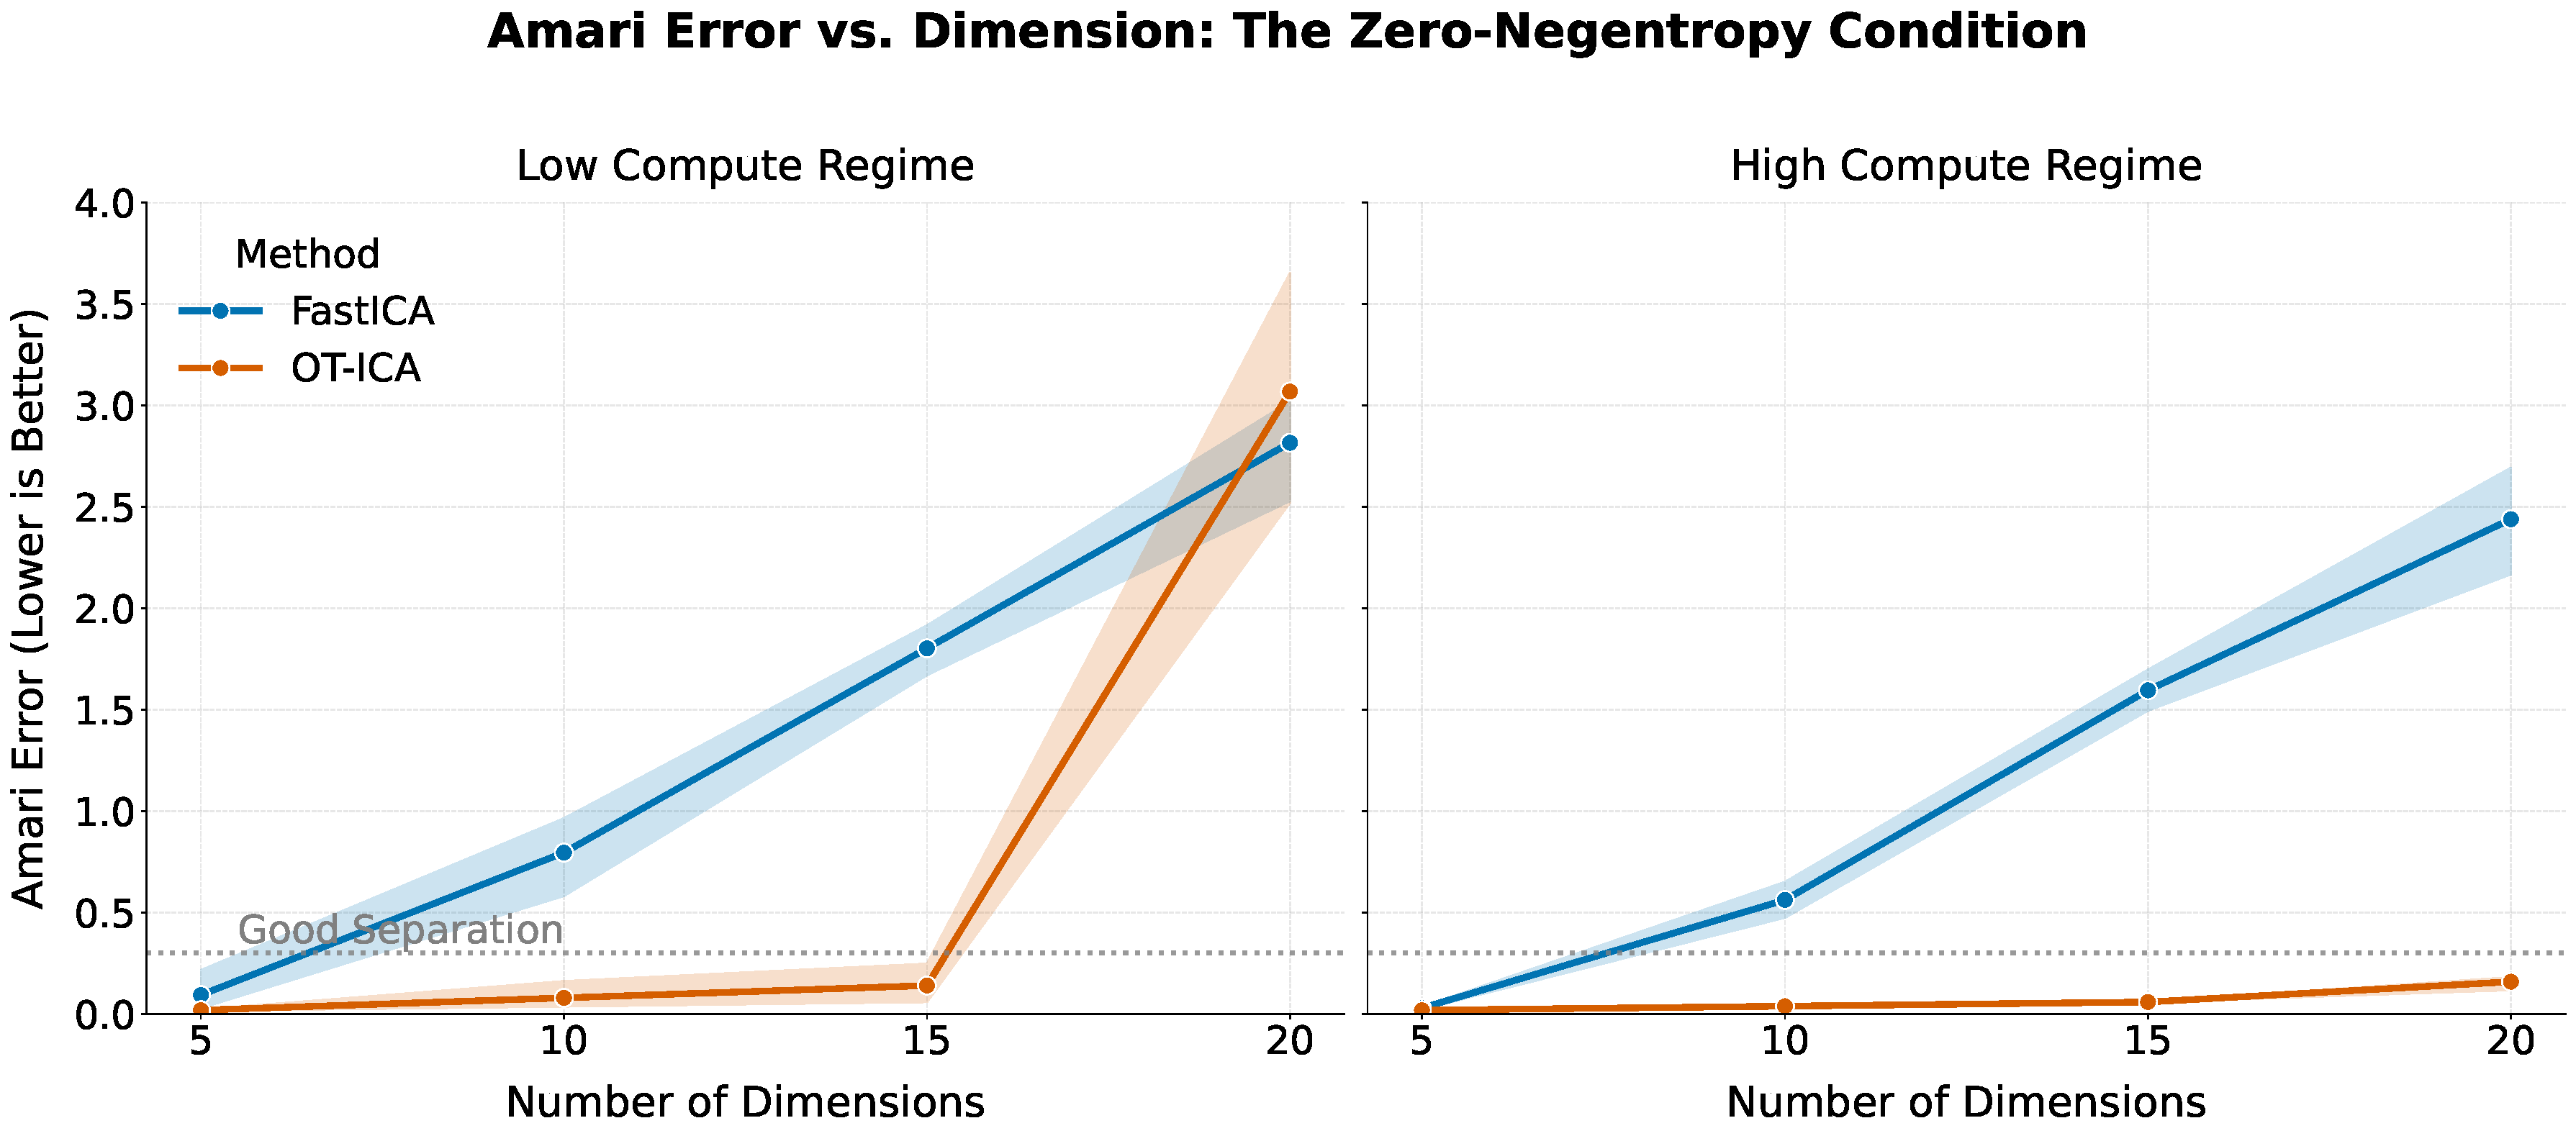
\includegraphics[width=0.75\textwidth]{zero_negentropy_amari_compute.pdf}
    \caption{Amari error comparison for the engineered zero-negentropy distribution. While FastICA fails completely for $d > 5$, OT-ICA reliably maintains separation across higher dimensions.}
\end{figure}

\subsection{The Vanishing Curvature Condition}
FastICA utilizes a Newton (second-order) fixed-point iteration. Defining $g(x) = G'(x)$ and $g'(x) = G''(x)$, FastICA approximates the Hessian matrix dynamically. For a given component $i$, the diagonal entry scales according to the expectation $\mathbf{H}_{ii} \approx \mathbb{E}\big[s_i g(s_i) - g'(s_i)\big]$.

The Newton update requires applying the inverse of this Hessian ($\mathbf{H}^{-1}$). If a non-Gaussian source distribution causes the expectation in the denominator to evaluate to zero, the inverse becomes mathematically undefined. This analytical divide-by-zero error makes the update step intractable. 

\begin{figure}[htbp]
    \centering
    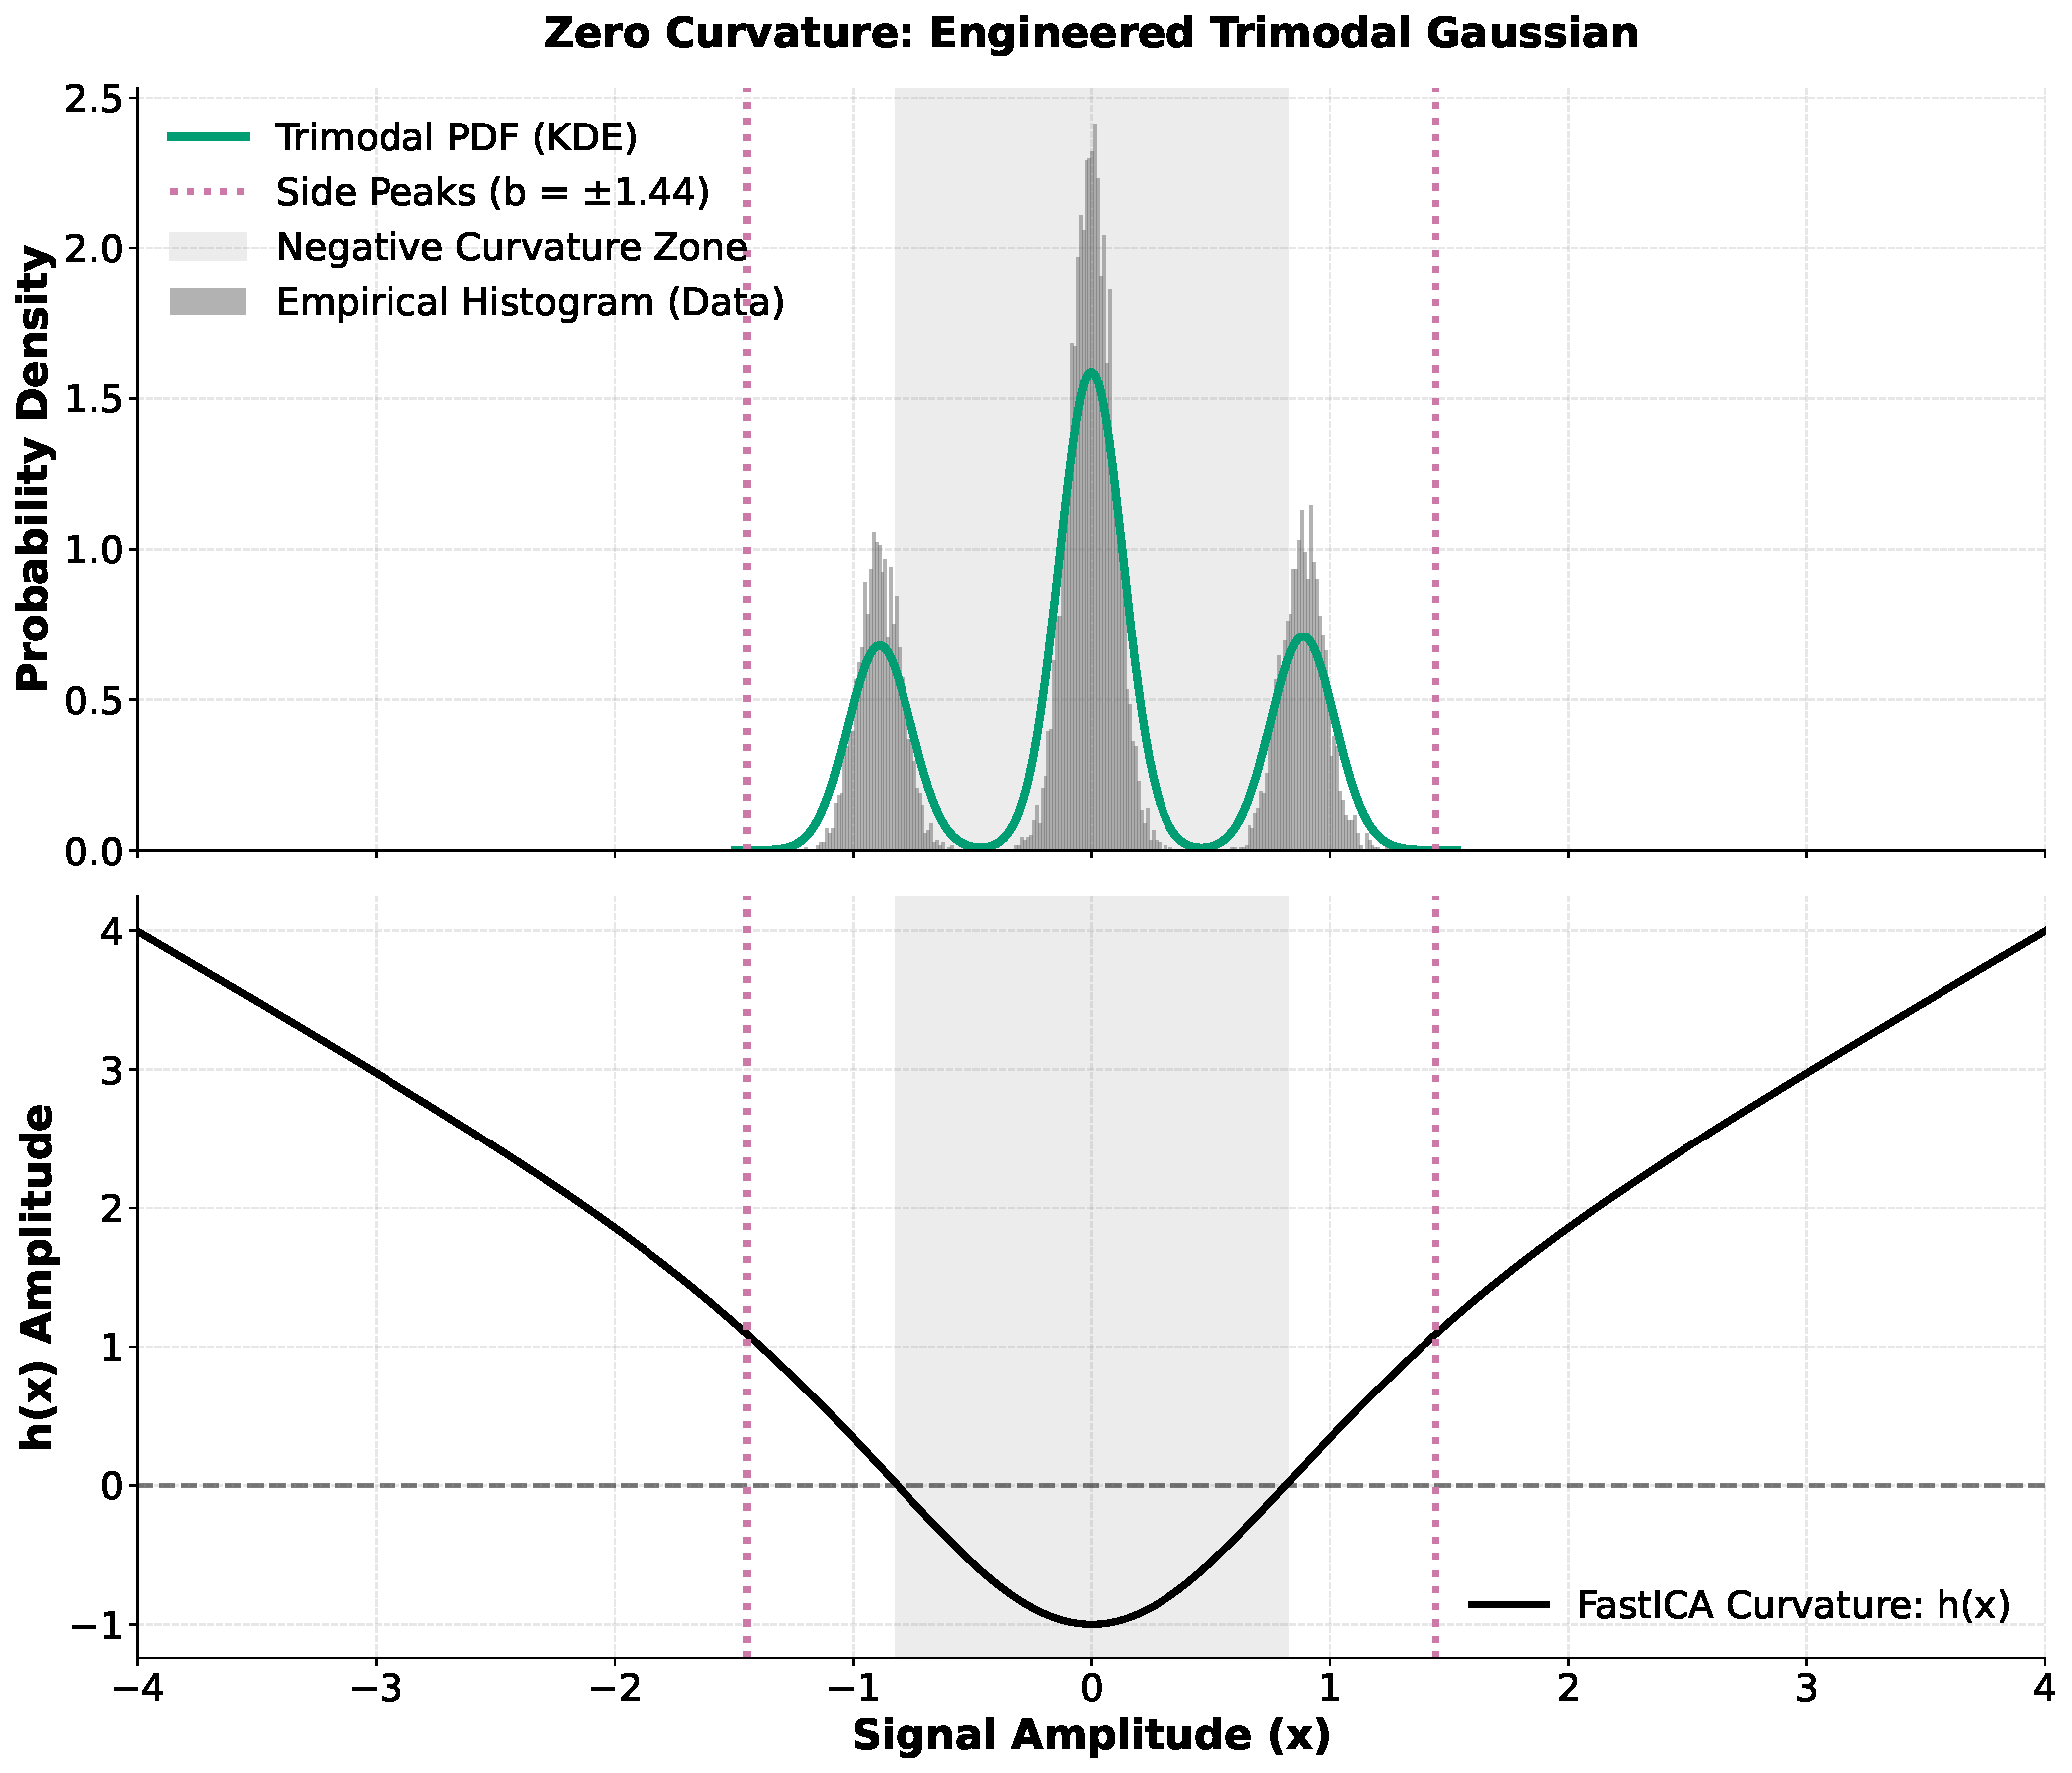
\includegraphics[width=0.75\textwidth]{vanishing_curvature_trimodal_pdf.pdf}
    \caption{The Vanishing Curvature Counterexample. The central mass generates negative algorithmic curvature, while the side peaks generate positive algorithmic curvature. We solved for parameters such that these regions precisely cancel while maintaining unit variance.}
\end{figure}

\begin{figure}[htbp]
    \centering
    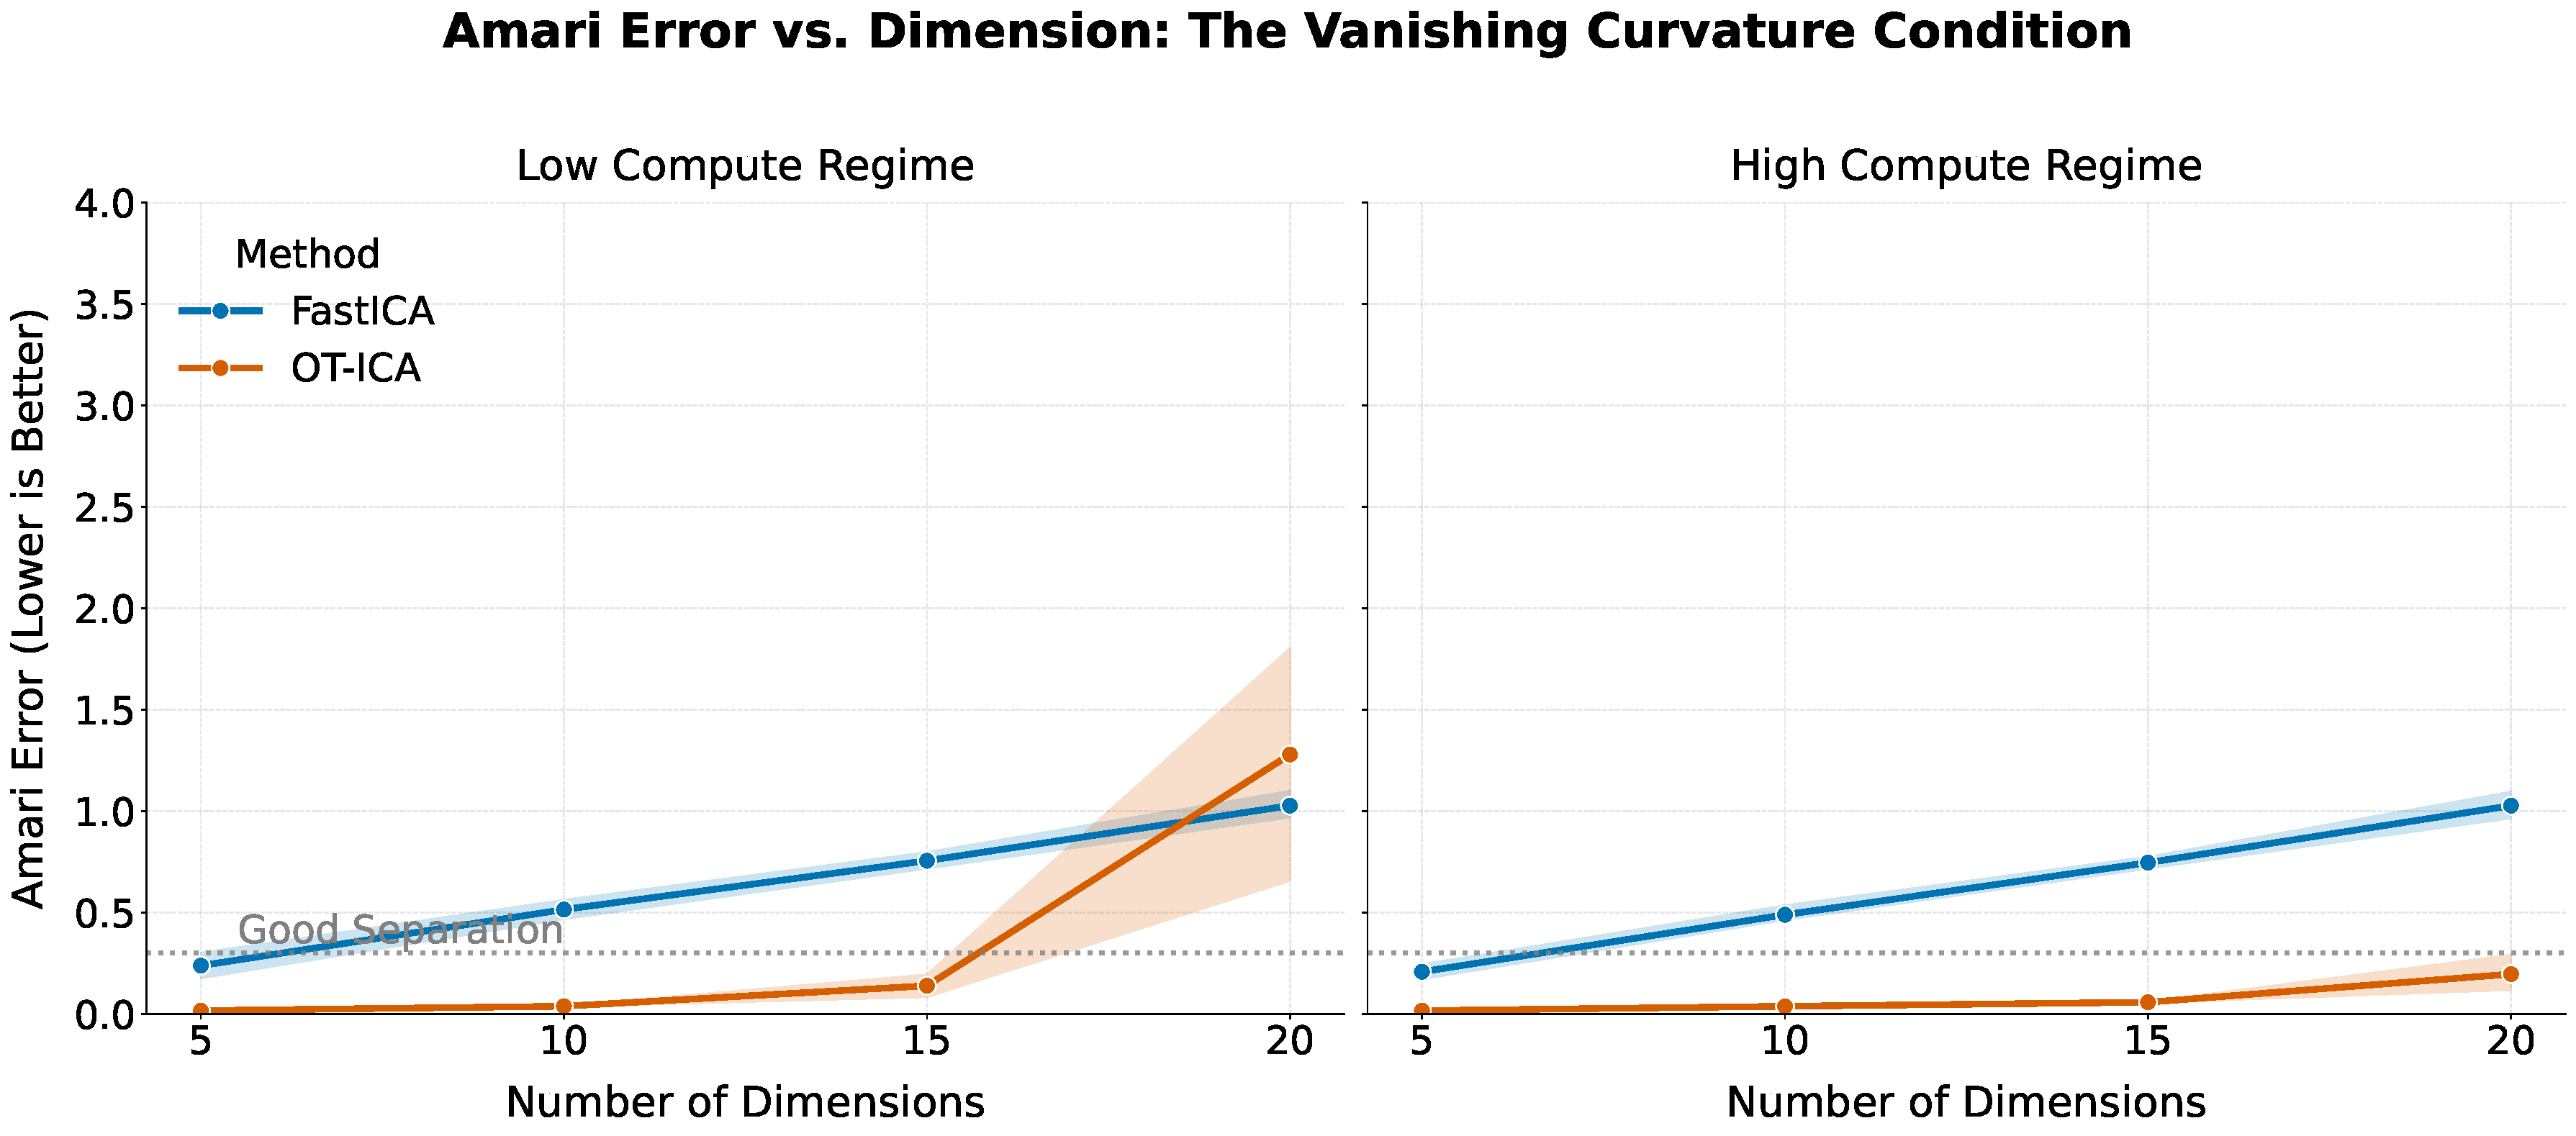
\includegraphics[width=0.75\textwidth]{vanishing_curvature_amari_compute.pdf}
    \caption{Amari error comparison for the zero-curvature distribution. FastICA fails entirely for $d \ge 10$. OT-ICA, utilizing the L-BFGS Quasi-Newton solver and the exact $W_2^2$ metric, bypasses the Hessian requirement and successfully maintains separation.}
\end{figure}

\section{Computational Scaling and Dimensionality Limits}
\label{app:scaling}

We benchmarked OT-ICA against FastICA using a linear mixture of continuous Laplace sources across increasing dimensions with a fixed sample size of $N=10,000$.

\begin{figure}[htbp]
    \centering
    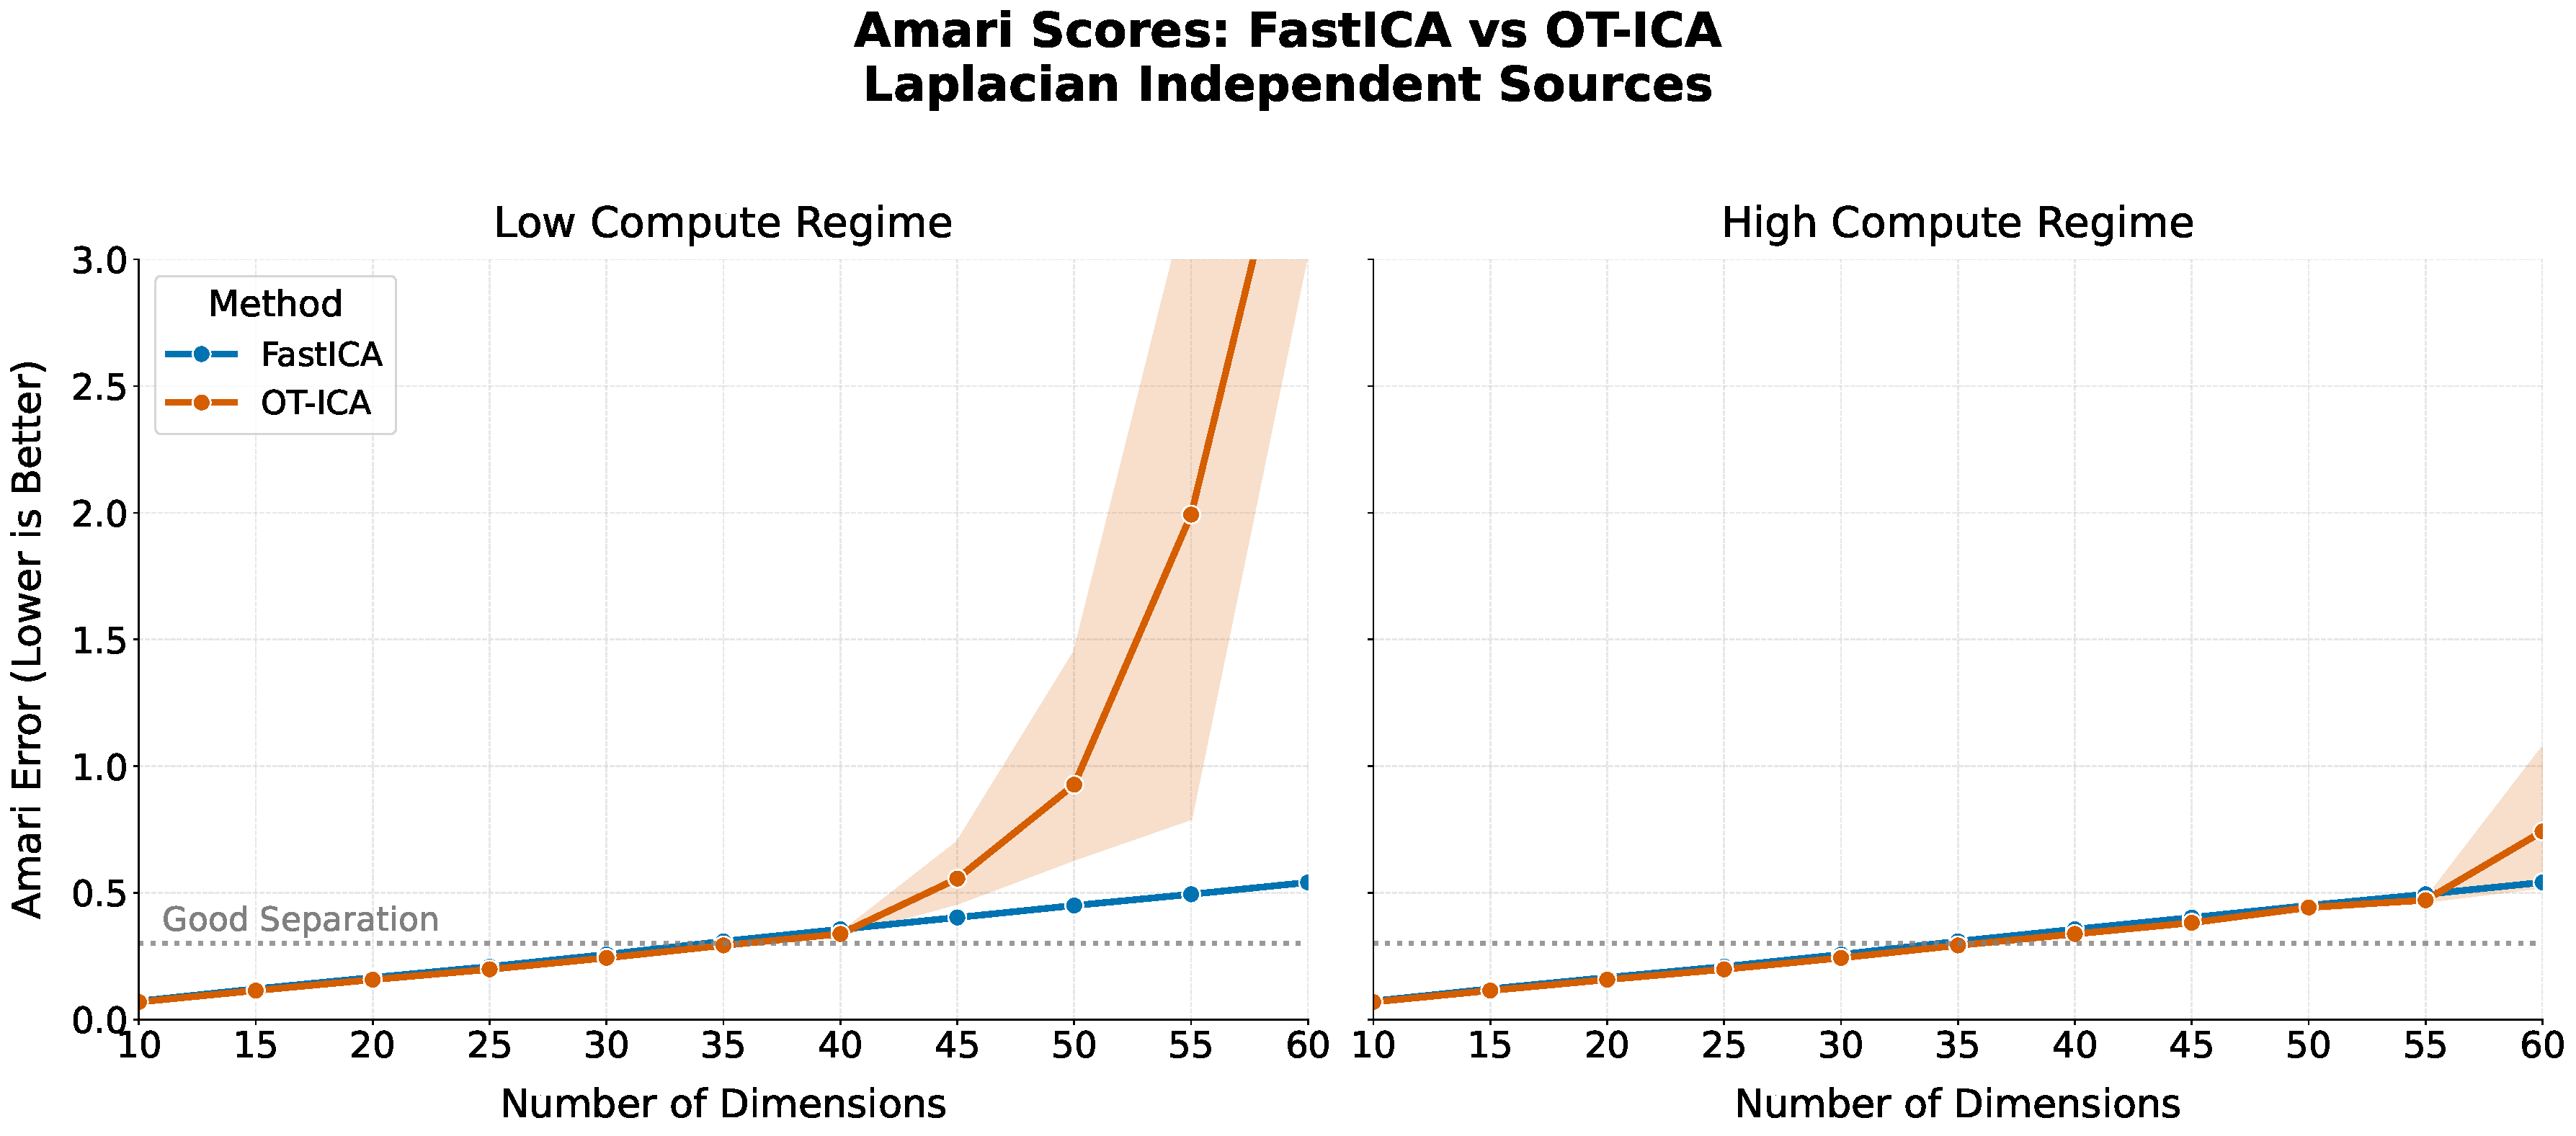
\includegraphics[width=0.75\textwidth]{laplace_amari_ot_ica_scaling.pdf}
    \caption{Amari error across dimensions for Laplacian sources at fixed $N=10{,}000$ samples. Both OT-ICA and FastICA hit the same curse-of-dimensionality noise ceiling at $d=40$---an artifact of finite-sample sparsity shared by all empirical ICA methods at this regime, not a deficiency specific to OT-ICA.}
\end{figure}

While OT-ICA maintains error rates comparable to FastICA ($E < 0.3$) in lower dimensions, both algorithms exhibit a loss in unmixing quality at $d=40$. This limit is a manifestation of the curse of dimensionality. The expected error of the empirical Wasserstein distance scales as $\mathcal{O}(N^{-1/d})$. As $d$ grows, a fixed finite sample fails to densely populate the state space, creating massive empty regions that swallow the gradient signal.

\begin{figure}[htbp]
    \centering
    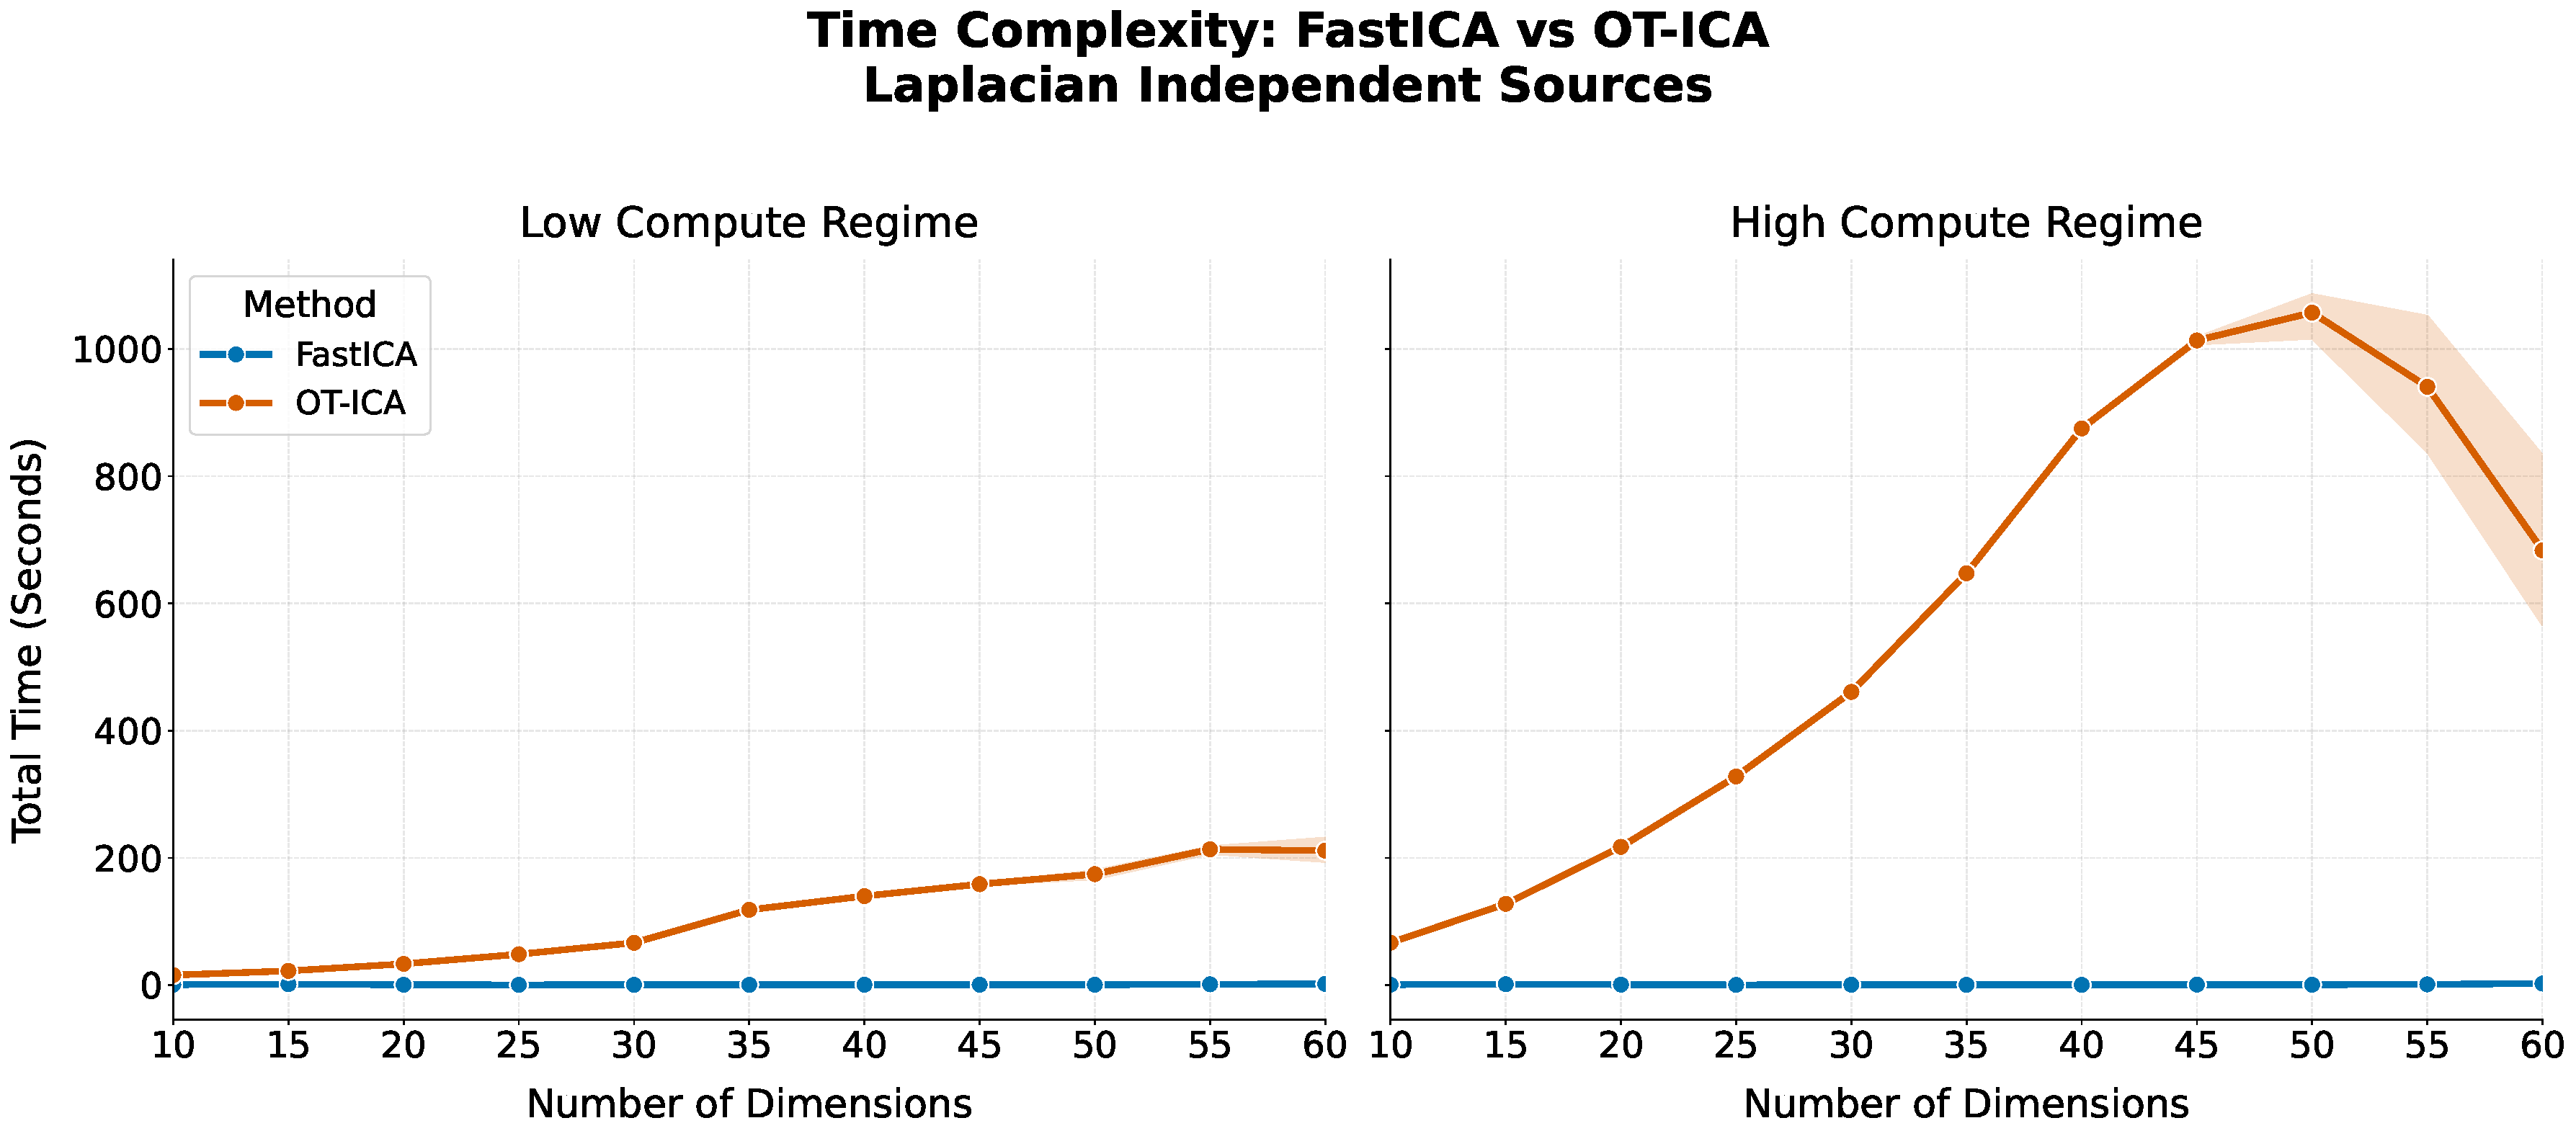
\includegraphics[width=0.75\textwidth]{laplace_time_ot_ica_scaling.pdf}
    \caption{Total execution time (in seconds) for FastICA and OT-ICA across dimensions.}
\end{figure}

The execution time for OT-ICA scales more steeply than FastICA. FastICA evaluates to $\mathcal{O}(d N)$ per iteration, making it computationally superior for exclusively homogeneous, continuous mixtures that do not trigger its proxy blind spots. OT-ICA incorporates parallel sorting across multiple restarts ($\mathcal{O}(K \cdot d N \log N)$), trading execution speed for geometric robustness on complex topologies.

\end{document}